% !TEX root = ../main.tex

\chapter{Phase 2 - Exploratory Data Analysis}

The structured dataset created during Phase~1 serves as the basis for the exploratory analysis presented in this chapter. The objective of 
this phase is to answer the research questions introduced in Chapter~1 through descriptive statistical analyses of the collected Upwork job
postings. The results presented here describe the observed characteristics of the analysed dataset, while their broader interpretation and
practical implications are discussed in the following chapter.

Prior to addressing the individual research questions, each job was assigned to one or more predefined job categories using a rule-based
keyword matching approach. Four primary categories were considered throughout the analysis: Data Engineer, Data Analyst, Machine Learning and
Python Automation. The classification was performed by matching predefined keywords against the job title, description and original Upwork category. 
Certain keywords were treated as stronger indicators and therefore contributed a higher classification score, while jobs that did not satisfy the
minimum matching criterion were assigned to the category \textit{Other}.

The resulting classifications were stored as an additional attribute of the structured dataset, allowing every job to be associated with one or
more job categories. This enriched dataset provides the foundation for all subsequent analyses presented in this chapter, including the investigation of
job distributions, required technologies, technical skills and budget characteristics.

\section{Research Question 1}

\textbf{Question}

Which types of projects are most frequently posted?

\medskip

\textbf{Methodology}

Following the job classification procedure described at the beginning of this chapter, the project type of every classified job posting was extracted from
the structured dataset. Three project types were considered throughout the analysis: \textit{Ongoing project}, \textit{One-time project} and
\textit{Complex project}. The frequency of each project type was then calculated separately for every job category in order to identify differences in
project characteristics across the analysed Python-related freelance domains.

Figure~\ref{fig:rq1_category_distribution} presents the number of classified job in each job category,
while Figures~\ref{fig:rq1_data_analyst}--\ref{fig:rq1_python_automation} illustrate the distribution of project types within each category.

\begin{figure}[H]
    \centering

    % első ábra
    \begin{subfigure}{0.75\textwidth}
        \centering
        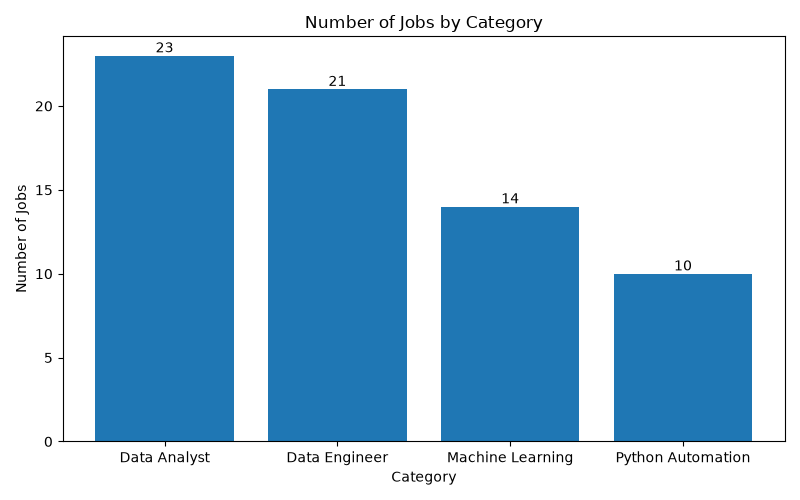
\includegraphics[width=\linewidth]{figures/diagrams/phase2/number_of_jobs_by_category.png}
        \caption{Number of classified jobs by job category.}
        \label{fig:rq1_category_distribution}
    \end{subfigure}

    \vspace{0.5cm}

    % második sor
    \begin{subfigure}{0.48\textwidth}
        \centering
        
\includegraphics[width=\linewidth]{figures/diagrams/phase2/data_analyst_project_types.png}
        \caption{Data Analyst}
        \label{fig:rq1_data_analyst}
    \end{subfigure}
    \hfill
    \begin{subfigure}{0.48\textwidth}
        \centering
        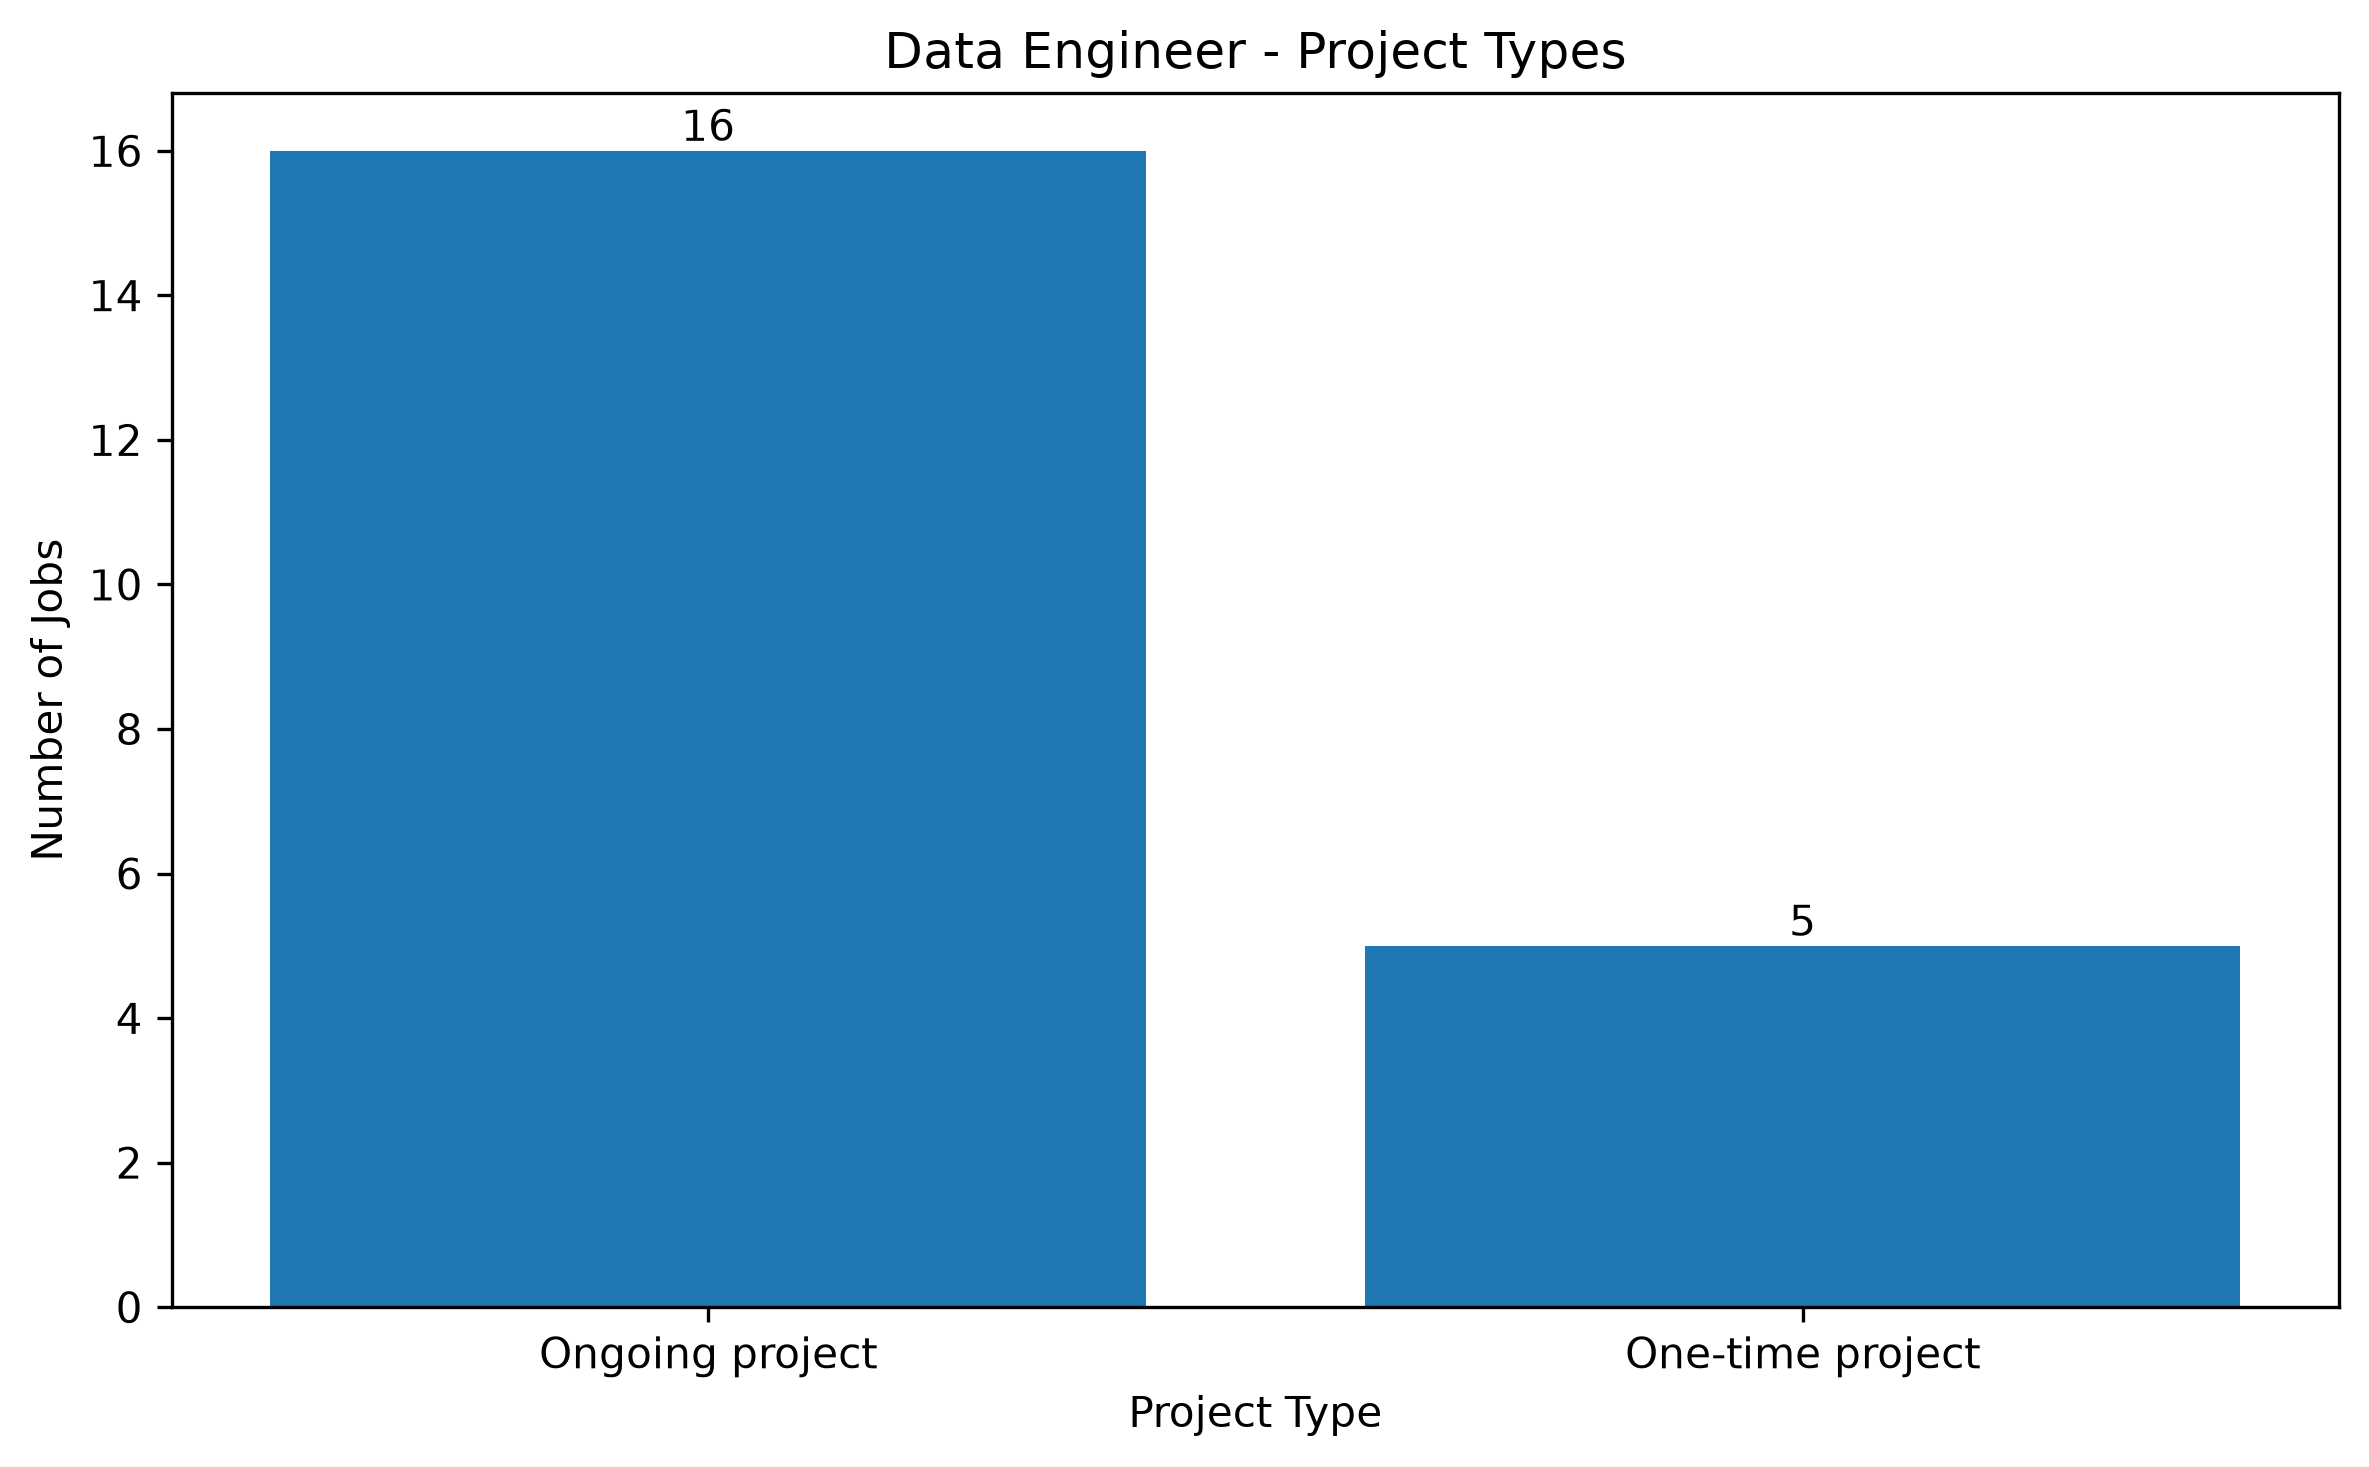
\includegraphics[width=\linewidth]{figures/diagrams/phase2/data_engineer_project_types.png}
        \caption{Data Engineer}
        \label{fig:rq1_data_engineer}
    \end{subfigure}

    \vspace{0.3cm}

    % harmadik sor
    \begin{subfigure}{0.48\textwidth}
        \centering
        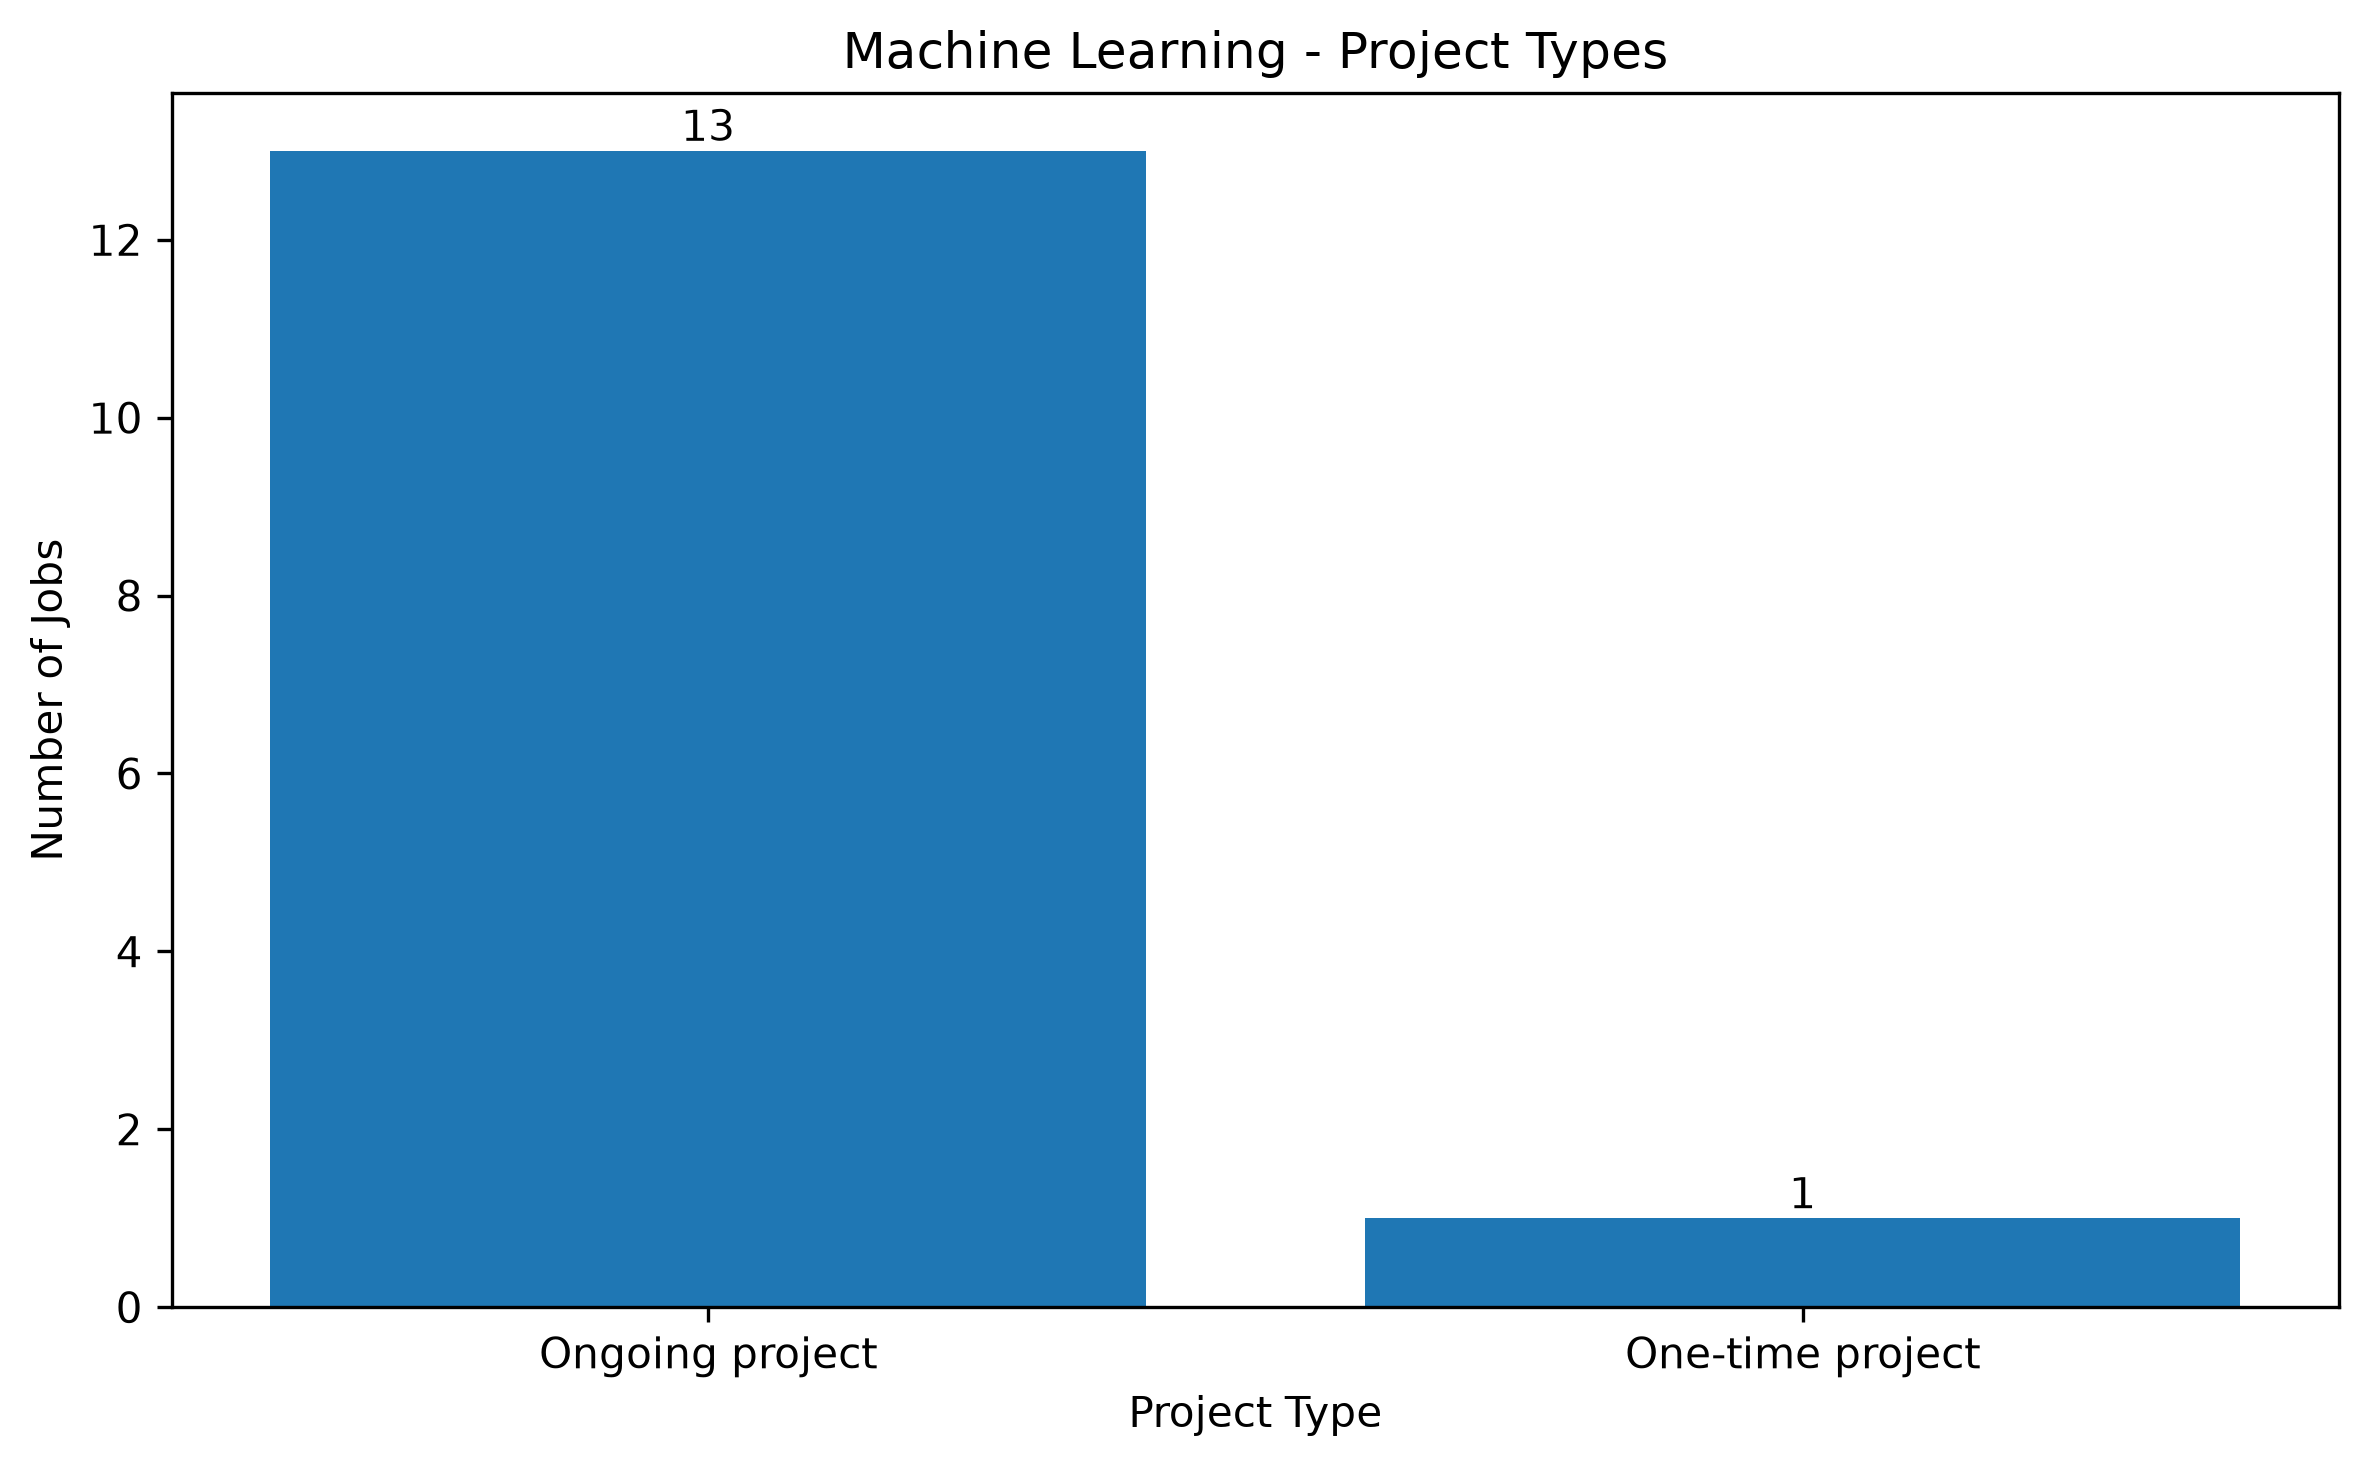
\includegraphics[width=\linewidth]{figures/diagrams/phase2/machine_learning_project_types.png}
        \caption{Machine Learning}
        \label{fig:rq1_machine_learning}
    \end{subfigure}
    \hfill
    \begin{subfigure}{0.48\textwidth}
        \centering
        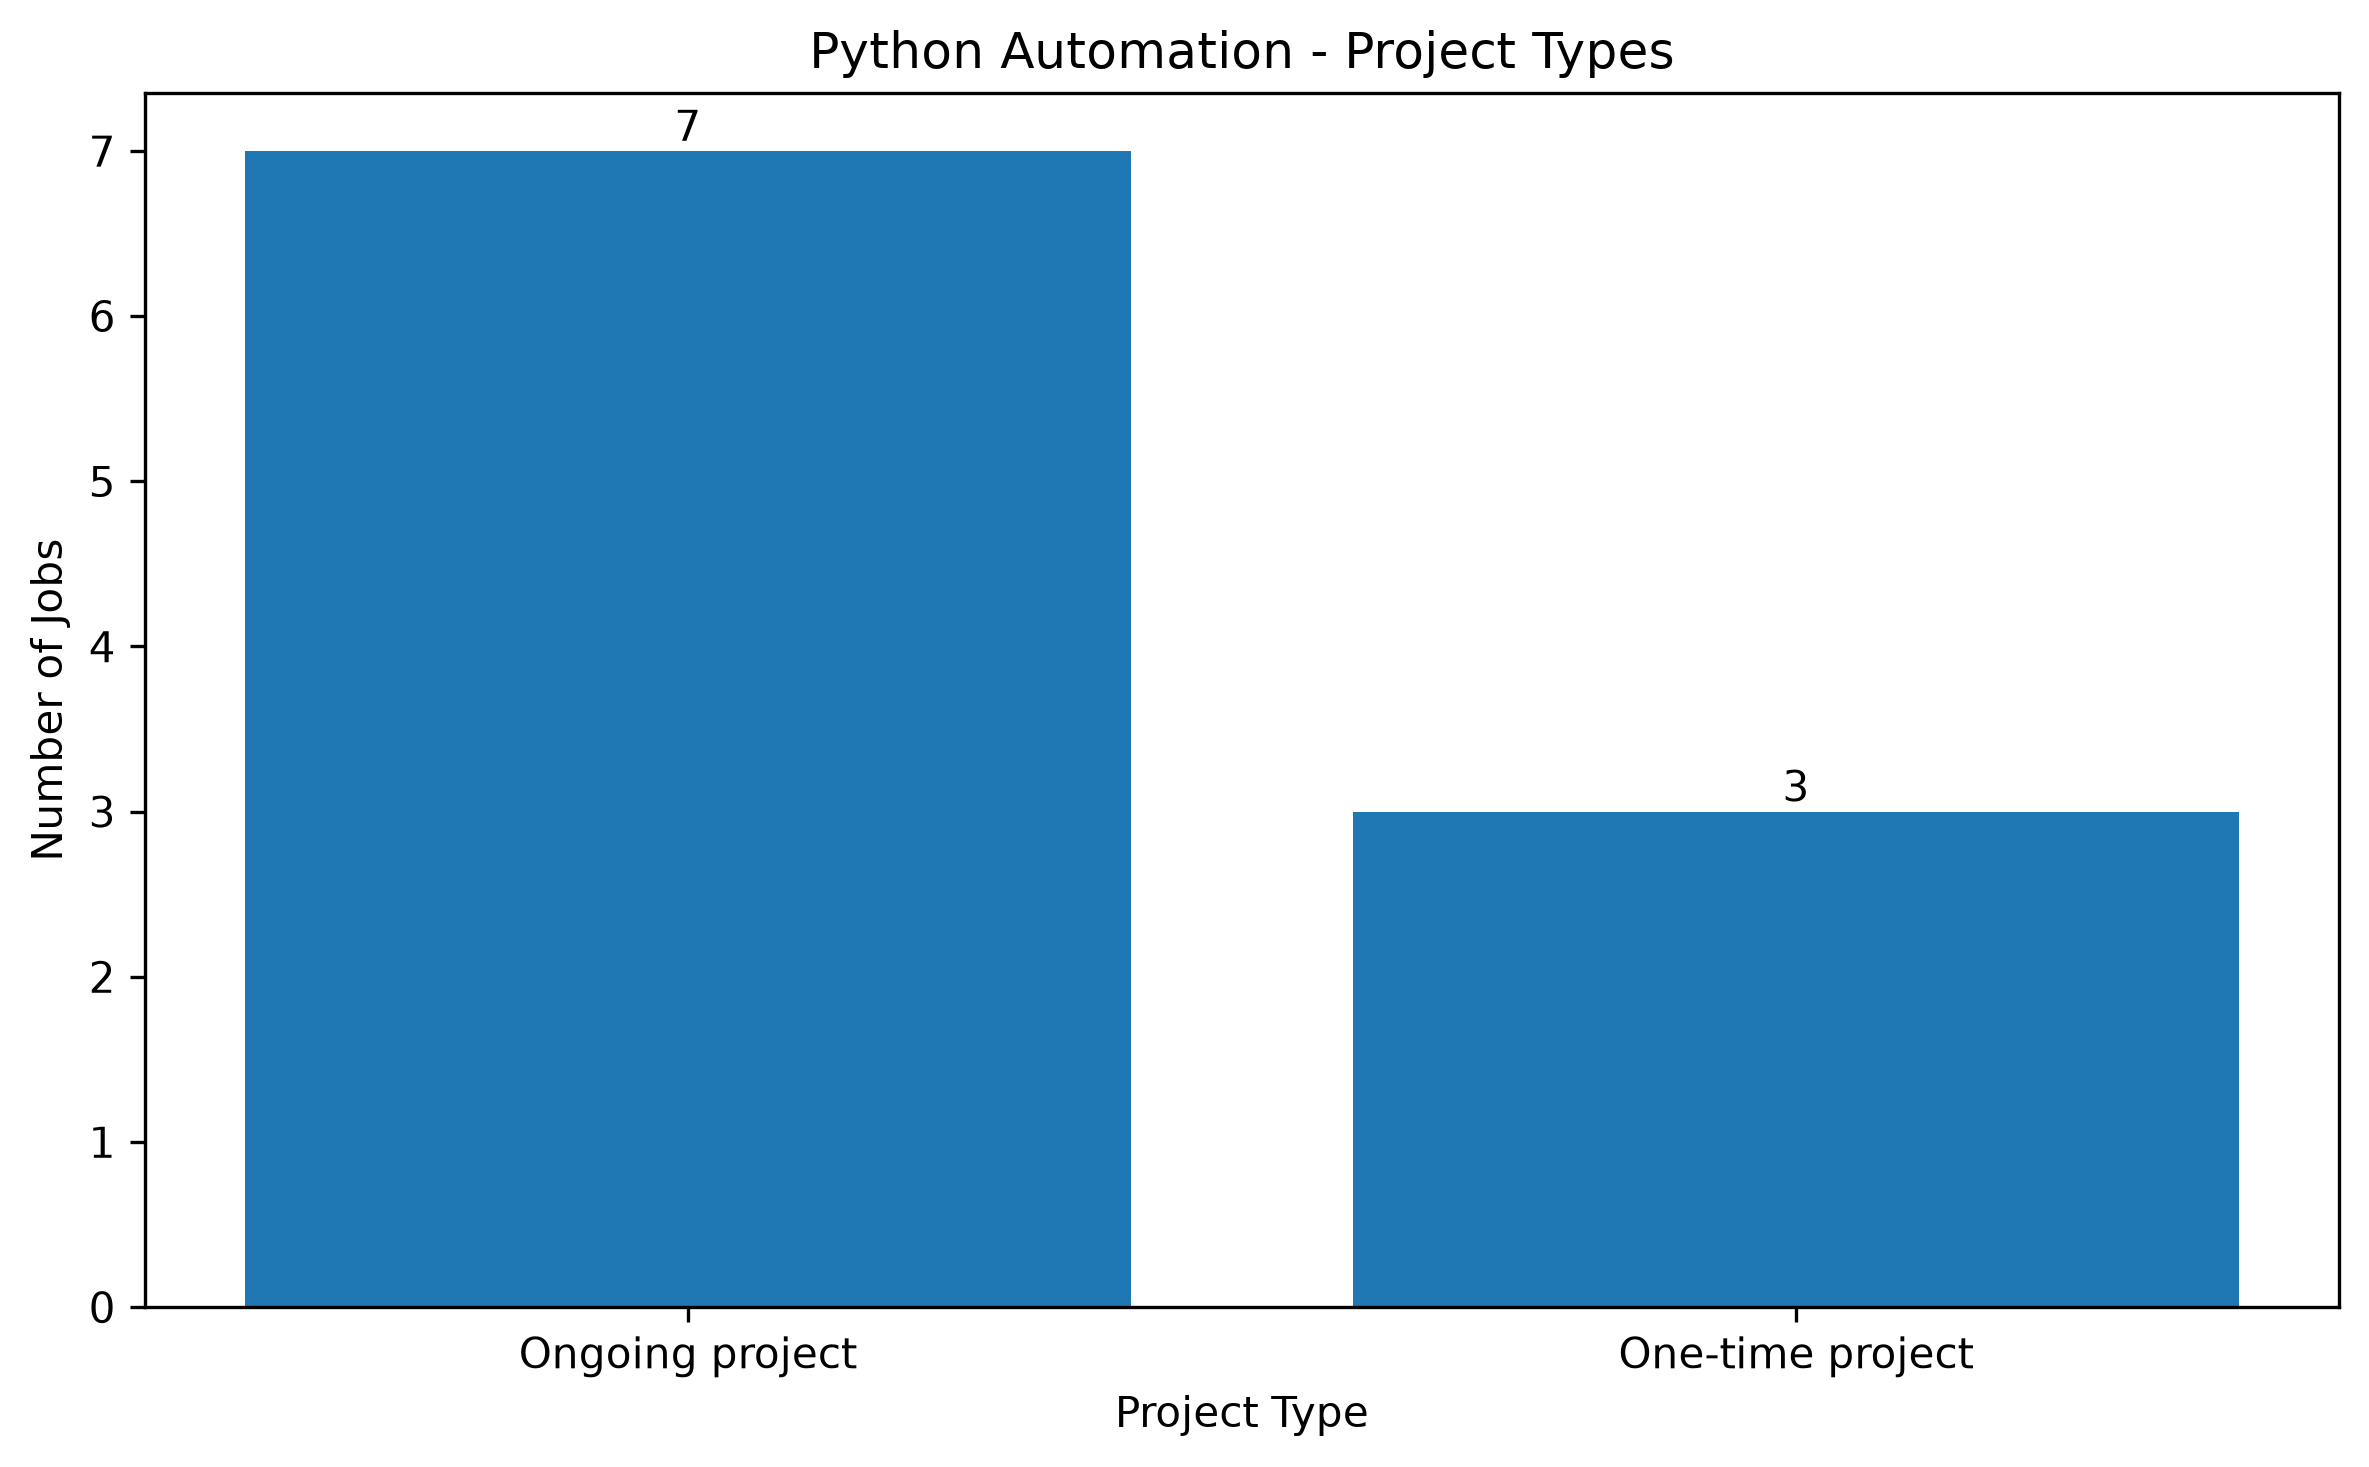
\includegraphics[width=\linewidth]{figures/diagrams/phase2/python_automation_project_types.png}
        \caption{Python Automation}
        \label{fig:rq1_python_automation}
    \end{subfigure}

    \caption{Distribution of job categories and project types within the analysed dataset. The complete numerical data used to generate these figures are available in
    \texttt{$/data/exports/tables/project-type-summary.csv$}}
    \label{fig:rq1_project_types}

\end{figure}

\medskip

\textbf{Results}

The classified dataset contains 23 Data Analyst, 21 Data Engineer, 14 Machine Learning and 10 Python Automation jobs
(Figure~\ref{fig:rq1_category_distribution}). Although the analysed dataset is relatively small, these distributions indicate that data-oriented freelance work is
primarily concentrated in the Data Analyst and Data Engineer categories.

Project type distributions reveal a clear preference for ongoing collaborations in most categories. Data Engineer jobs exhibit the strongest tendency towards
long-term engagements, with 16 ongoing projects compared to only 5 one-time projects. Machine Learning jobs show an even more pronounced pattern, where 13
out of 14 classified jobs correspond to ongoing work. Python Automation jobs follow a similar trend, consisting of 7 ongoing and 3 one-time projects.

Data Analyst jobs differ slightly from the other categories. While ongoing projects remain common, the numbers of ongoing and one-time projects are identical
(11 each), and one job was classified as a complex project. This makes Data Analyst the only analysed category containing all three project types.

\medskip

\textbf{Discussion}

The analysis suggests that long-term collaborations dominate the selected Python-related freelance market. This tendency is particularly pronounced for
Data Engineering and Machine Learning jobs, where clients appear to prefer sustained cooperation rather than isolated tasks. In contrast, Data Analyst projects
exhibit a more balanced distribution between ongoing and one-time engagements, indicating a broader variety of project scopes within this category.
These observations provide an initial overview of the analysed marketplace and establish the context for the subsequent investigation of required technologies,
Python libraries and technical skills.

\section{Research Question 2}

\textbf{Question}

Which Python libraries and frameworks are most commonly required?

\medskip

\textbf{Methodology}

The structured dataset was analysed to identify explicit references to Python libraries and frameworks in the job descriptions. Package names were
extracted using a predefined dictionary of commonly used Python libraries relevant to data analysis, data engineering, machine learning and
automation. Whenever a package was mentioned in a job description, it was counted once for that job, regardless of the number of occurrences within
the text.

To facilitate comparison between categories of different sizes, package frequencies were normalised by the number of classified jobs in each category
and expressed as percentages. Figure~\ref{fig:rq2_python_packages_overall} summarises the overall frequency of Python packages within the analysed dataset,
while the accompanying subfigures ~\ref{fig:rq2_python_packages_data_analyst}--\ref{fig:rq2_python_packages_python_automation} present the distributions separately for Data Analyst, Data Engineer, Machine Learning and Python Automation jobss.

\begin{figure}[H]
    \centering

    % első ábra
    \begin{subfigure}{0.75\textwidth}
        \centering
        
\includegraphics[width=\linewidth]{figures/diagrams/phase2/most_requested_python_packages_overall.png}
        \caption{Overall frequency of Python packages.}
        \label{fig:rq2_python_packages_overall}
    \end{subfigure}

    \vspace{0.5cm}

    % második sor
    \begin{subfigure}{0.48\textwidth}
        \centering
        
\includegraphics[width=\linewidth]{figures/diagrams/phase2/data_analyst_most_requested_python_packages.png}
        \caption{Data Analyst}
        \label{fig:rq2_python_packages_data_analyst}
    \end{subfigure}
    \hfill
    \begin{subfigure}{0.48\textwidth}
        \centering
        
\includegraphics[width=\linewidth]{figures/diagrams/phase2/data_engineer_most_requested_python_packages.png}
        \caption{Data Engineer}
        \label{fig:rq2_python_packages_data_engineer}
    \end{subfigure}

    \vspace{0.3cm}

    % harmadik sor
    \begin{subfigure}{0.48\textwidth}
        \centering
        
\includegraphics[width=\linewidth]{figures/diagrams/phase2/machine_learning_most_requested_python_packages.png}
        \caption{Machine Learning}
        \label{fig:rq2_python_packages_machine_learning}
    \end{subfigure}
    \hfill
    \begin{subfigure}{0.48\textwidth}
        \centering
        
\includegraphics[width=\linewidth]{figures/diagrams/phase2/python_automation_most_requested_python_packages.png}
        \caption{Python Automation}
        \label{fig:rq2_python_packages_python_automation}
    \end{subfigure}

    \caption{Frequency of Python libraries and frameworks within the analysed dataset, overall and by job category. The complete numerical data
    used to generate these figures are available in \texttt{$/data/exports/tables/python-package-summary.csv$}}
    \label{fig:rq2_python_packages}
    
\end{figure}

\medskip

\textbf{Results}

Across the complete dataset, Pandas is by far the most frequently requested Python package, appearing in approximately 32\% of
all analysed job postings. NumPy represents the second most common library (approximately 16\%), followed by Matplotlib (9\%) and
scikit-learn (5\%). All remaining packages occur only occasionally, each appearing in fewer than 3\% of the analysed jobs.

Although Pandas dominates every analysed category, noticeable differences emerge between specialisations. Machine Learning jobs exhibit
the broadest collection of requested libraries, with frequent mentions of NumPy, scikit-learn, Matplotlib, OpenCV, XGBoost and LightGBM.
Data Analyst jobs show a similar but slightly more analysis-oriented profile, where Pandas and NumPy dominate, accompanied by
visualisation libraries such as Matplotlib, Seaborn and Plotly.

Data Engineering jobs rely overwhelmingly on Pandas, while the remaining libraries appear only sporadically. Python Automation jobs display
the narrowest technology profile, where Pandas is accompanied primarily by browser automation libraries such as Selenium and Playwright.

\medskip

\textbf{Discussion}

The results indicate that Pandas constitutes the fundamental Python library across all analysed freelance domains, regardless of job specialisation.
NumPy also appears consistently, particularly in jobs involving data analysis and machine learning, confirming its role as one of
the core scientific computing libraries within the Python ecosystem.

The greater diversity of requested libraries in Machine Learning jobs reflects the wider range of technical tasks typically associated with
this domain, including data processing, model development and computer vision. In contrast, Data Engineering and Python Automation jobs tend to
require a smaller and more specialised collection of libraries. These observations provide an initial indication of which Python packages should be
prioritised when preparing for different segments of the freelance market.

\section{Research Question 3}

\textbf{Question}

Which technologies and software tools are most frequently required?

\medskip

\textbf{Methodology}

The extraction of technologies and software tools followed the same rule-based approach used for Python package identification in the previous
research question. A predefined keyword dictionary was created containing  programming languages, database systems, business intelligence software,
cloud platforms, AI tools, web technologies and other commonly requested technical skills. Each collected job description was automatically scanned,
and every detected technology was recorded.

The extracted technologies were subsequently aggregated both across the entire dataset and within each job category. Their relative frequencies were
calculated as the percentage of job postings mentioning each technology. The overall technology distribution and the category-specific distributions
are presented in Figure~\ref{fig:rq3_technologies}, while the similarities and differences between job categories are further illustrated using
the heat mapshown in Figure~\ref{fig:rq3_technology_heatmap}.

\begin{figure}[H]
    \centering

    % első ábra
    \begin{subfigure}{0.75\textwidth}
        \centering
        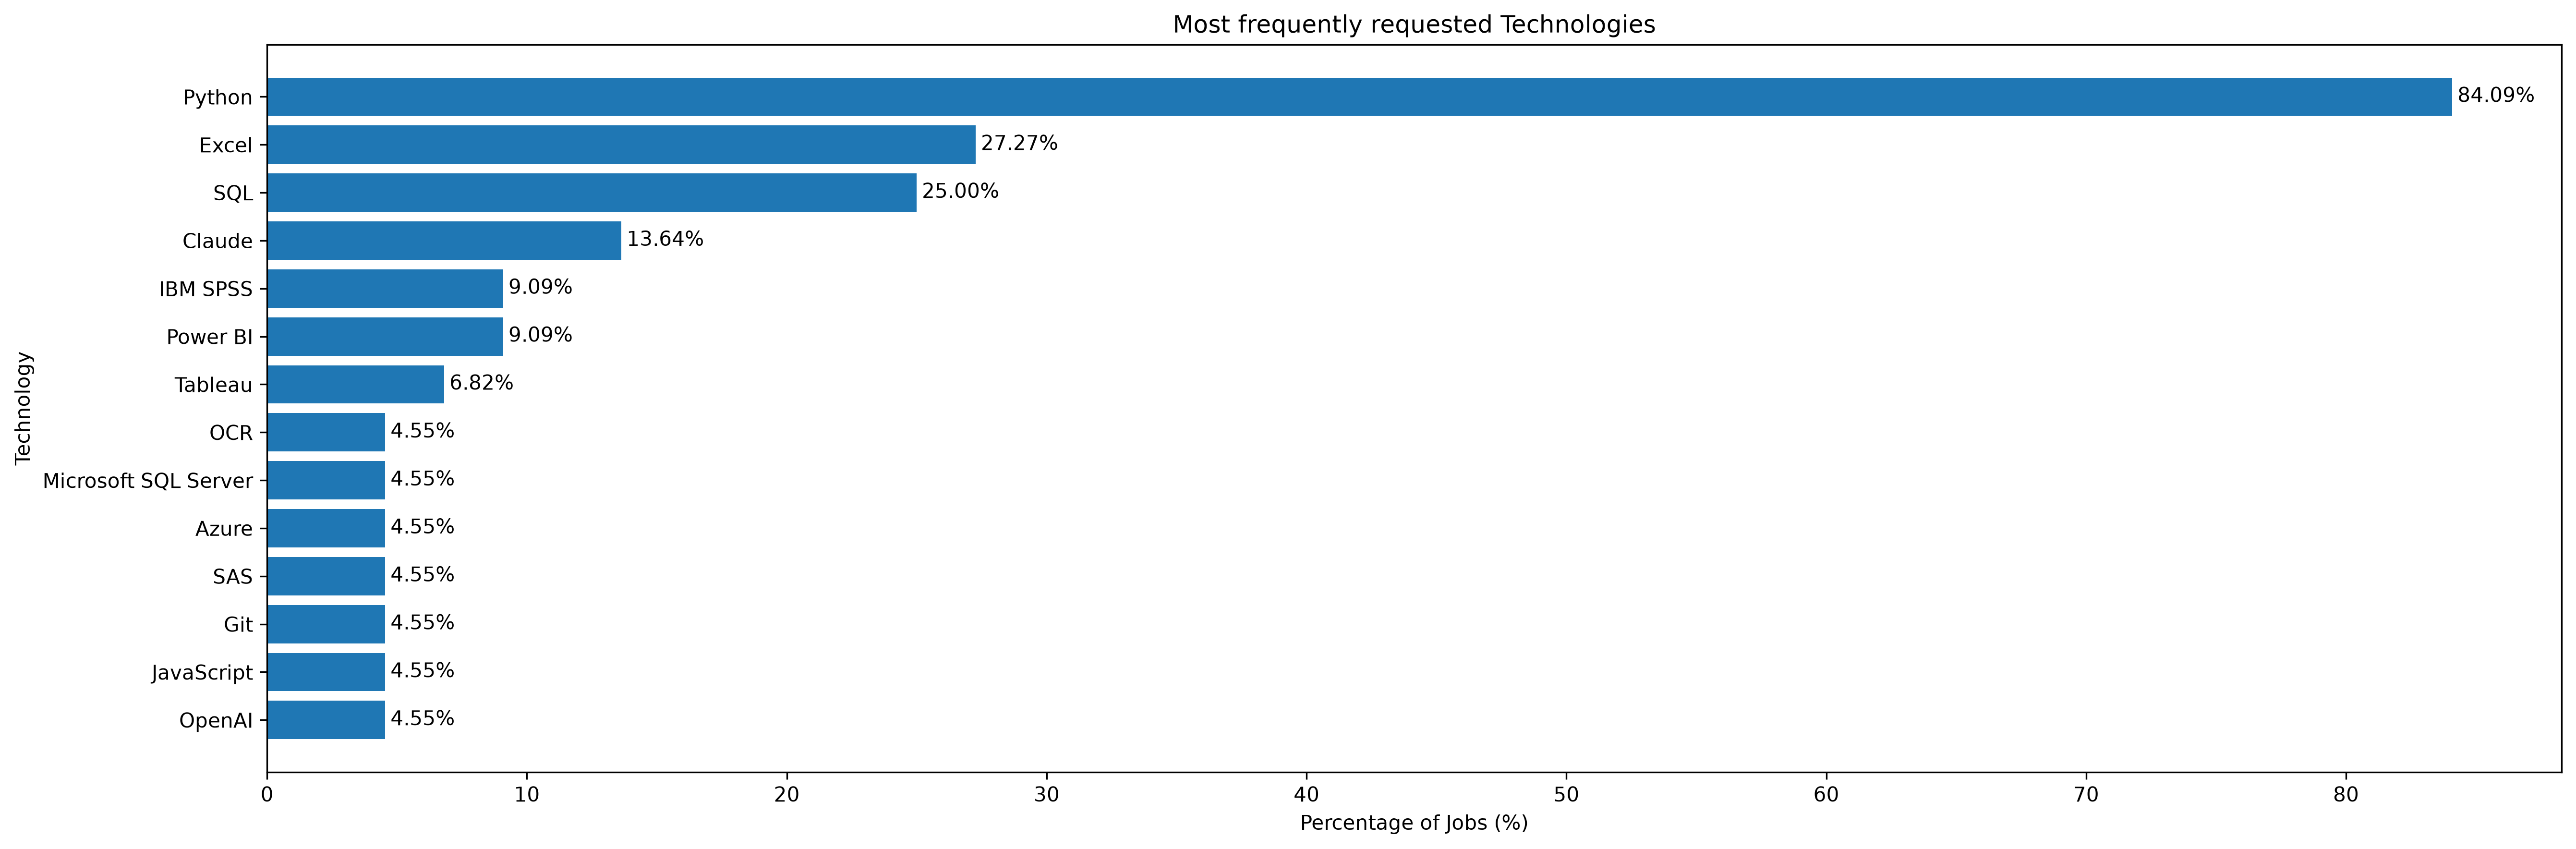
\includegraphics[width=\linewidth]{figures/diagrams/phase2/most_requested_technologies_overall.png}
        \caption{Overall frequency of technologies and tools.}
        \label{fig:rq3_technologies_overall}
    \end{subfigure}

    \vspace{0.5cm}

    % második sor
    \begin{subfigure}{0.48\textwidth}
        \centering
        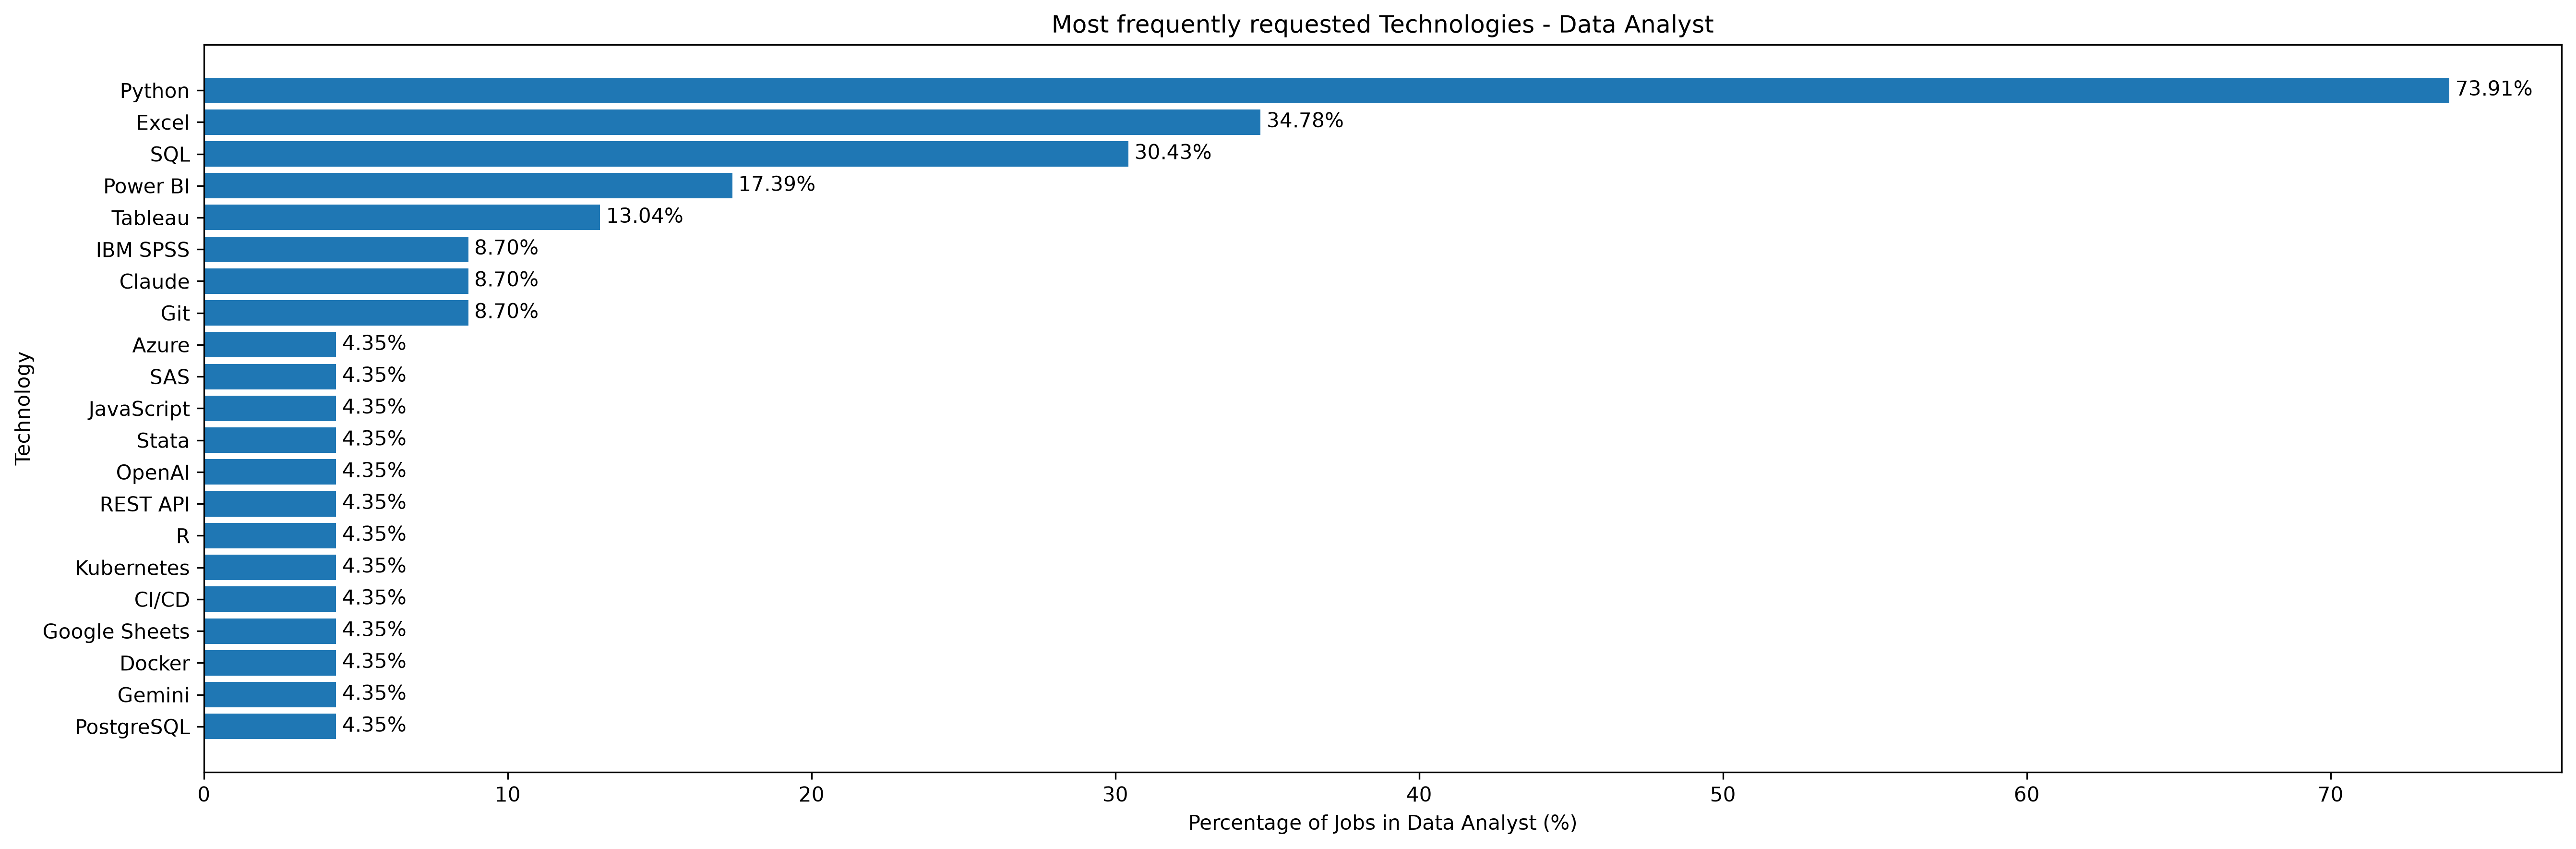
\includegraphics[width=\linewidth]{figures/diagrams/phase2/data_analyst_most_requested_technologies.png}
        \caption{Data Analyst}
        \label{fig:rq3_technologies_data_analyst}
    \end{subfigure}
    \hfill
    \begin{subfigure}{0.48\textwidth}
        \centering
        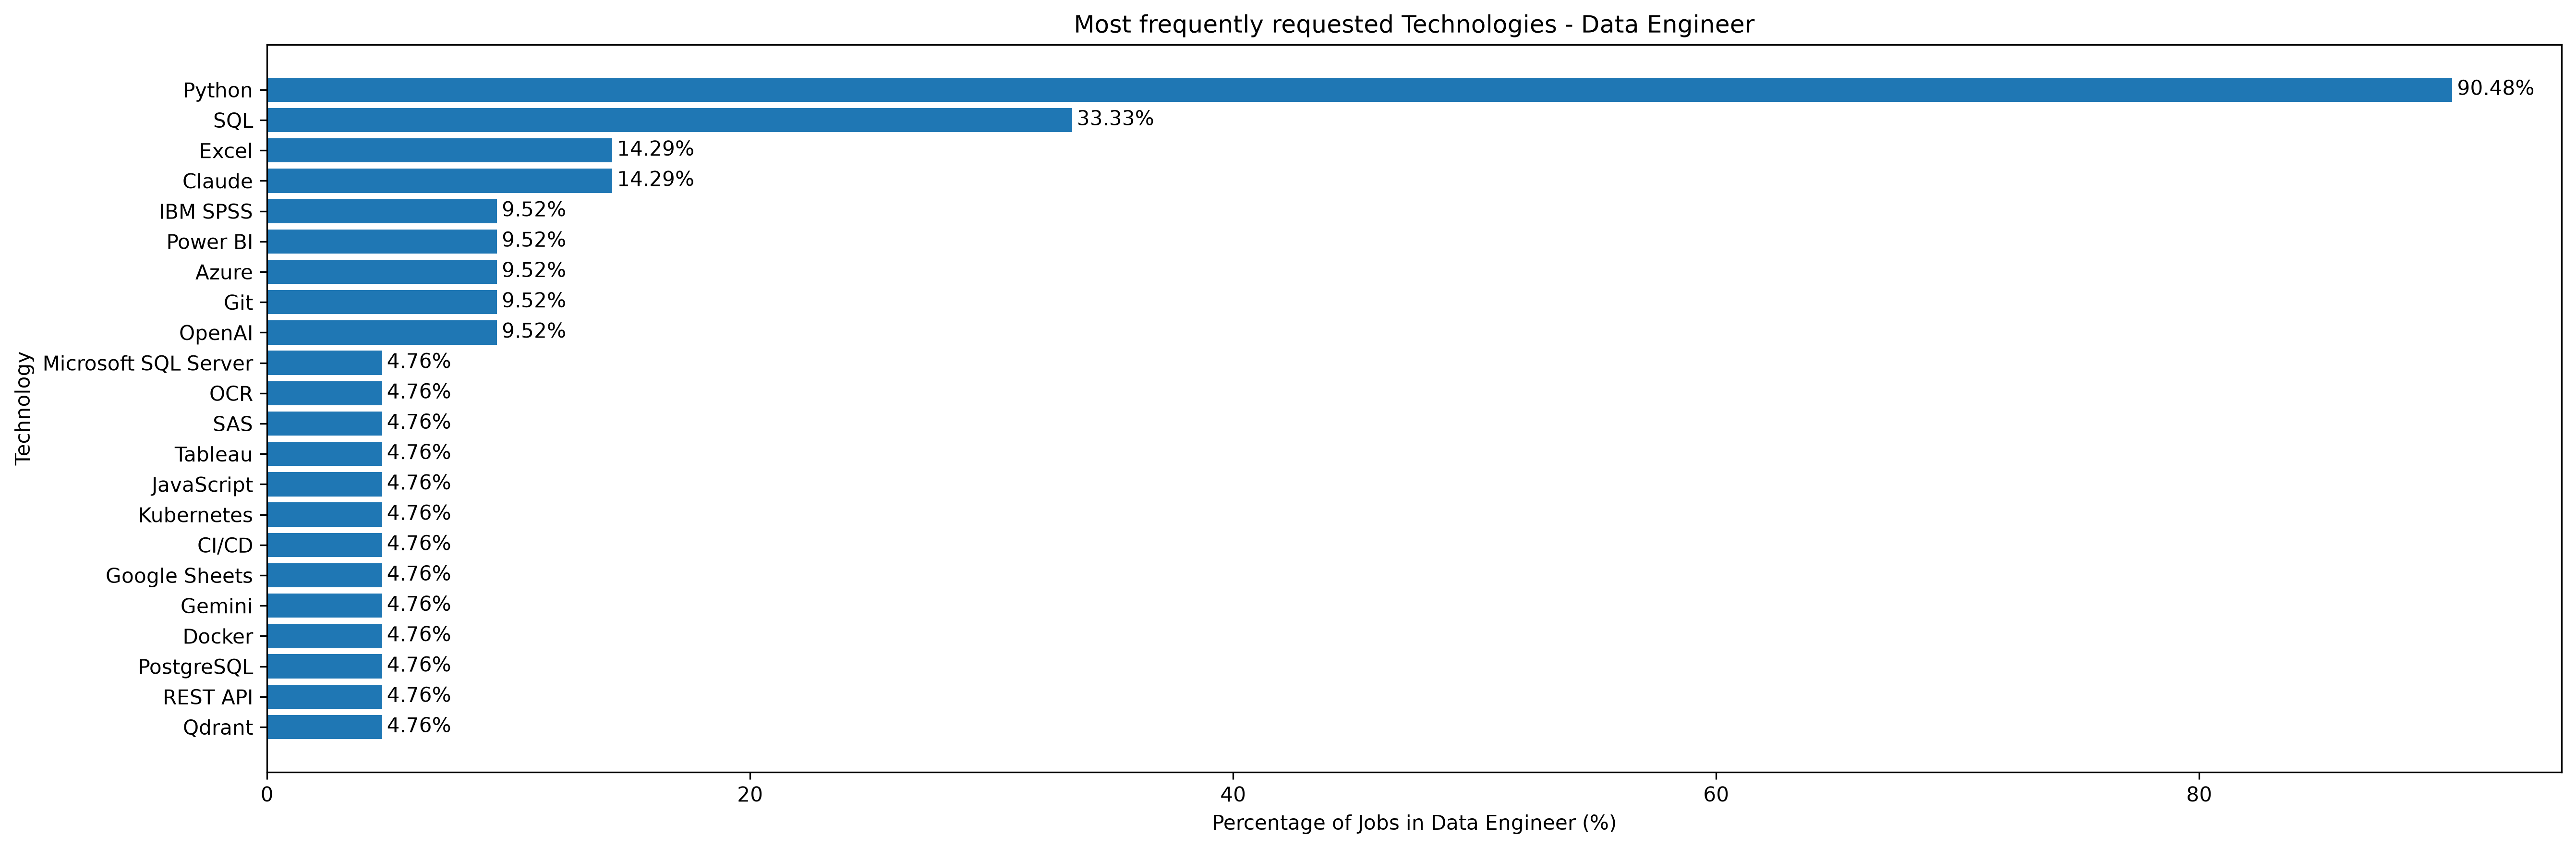
\includegraphics[width=\linewidth]{figures/diagrams/phase2/data_engineer_most_requested_technologies.png}
        \caption{Data Engineer}
        \label{fig:rq3_technologies_data_engineer}
    \end{subfigure}

    \vspace{0.3cm}

    % harmadik sor
    \begin{subfigure}{0.48\textwidth}
        \centering
        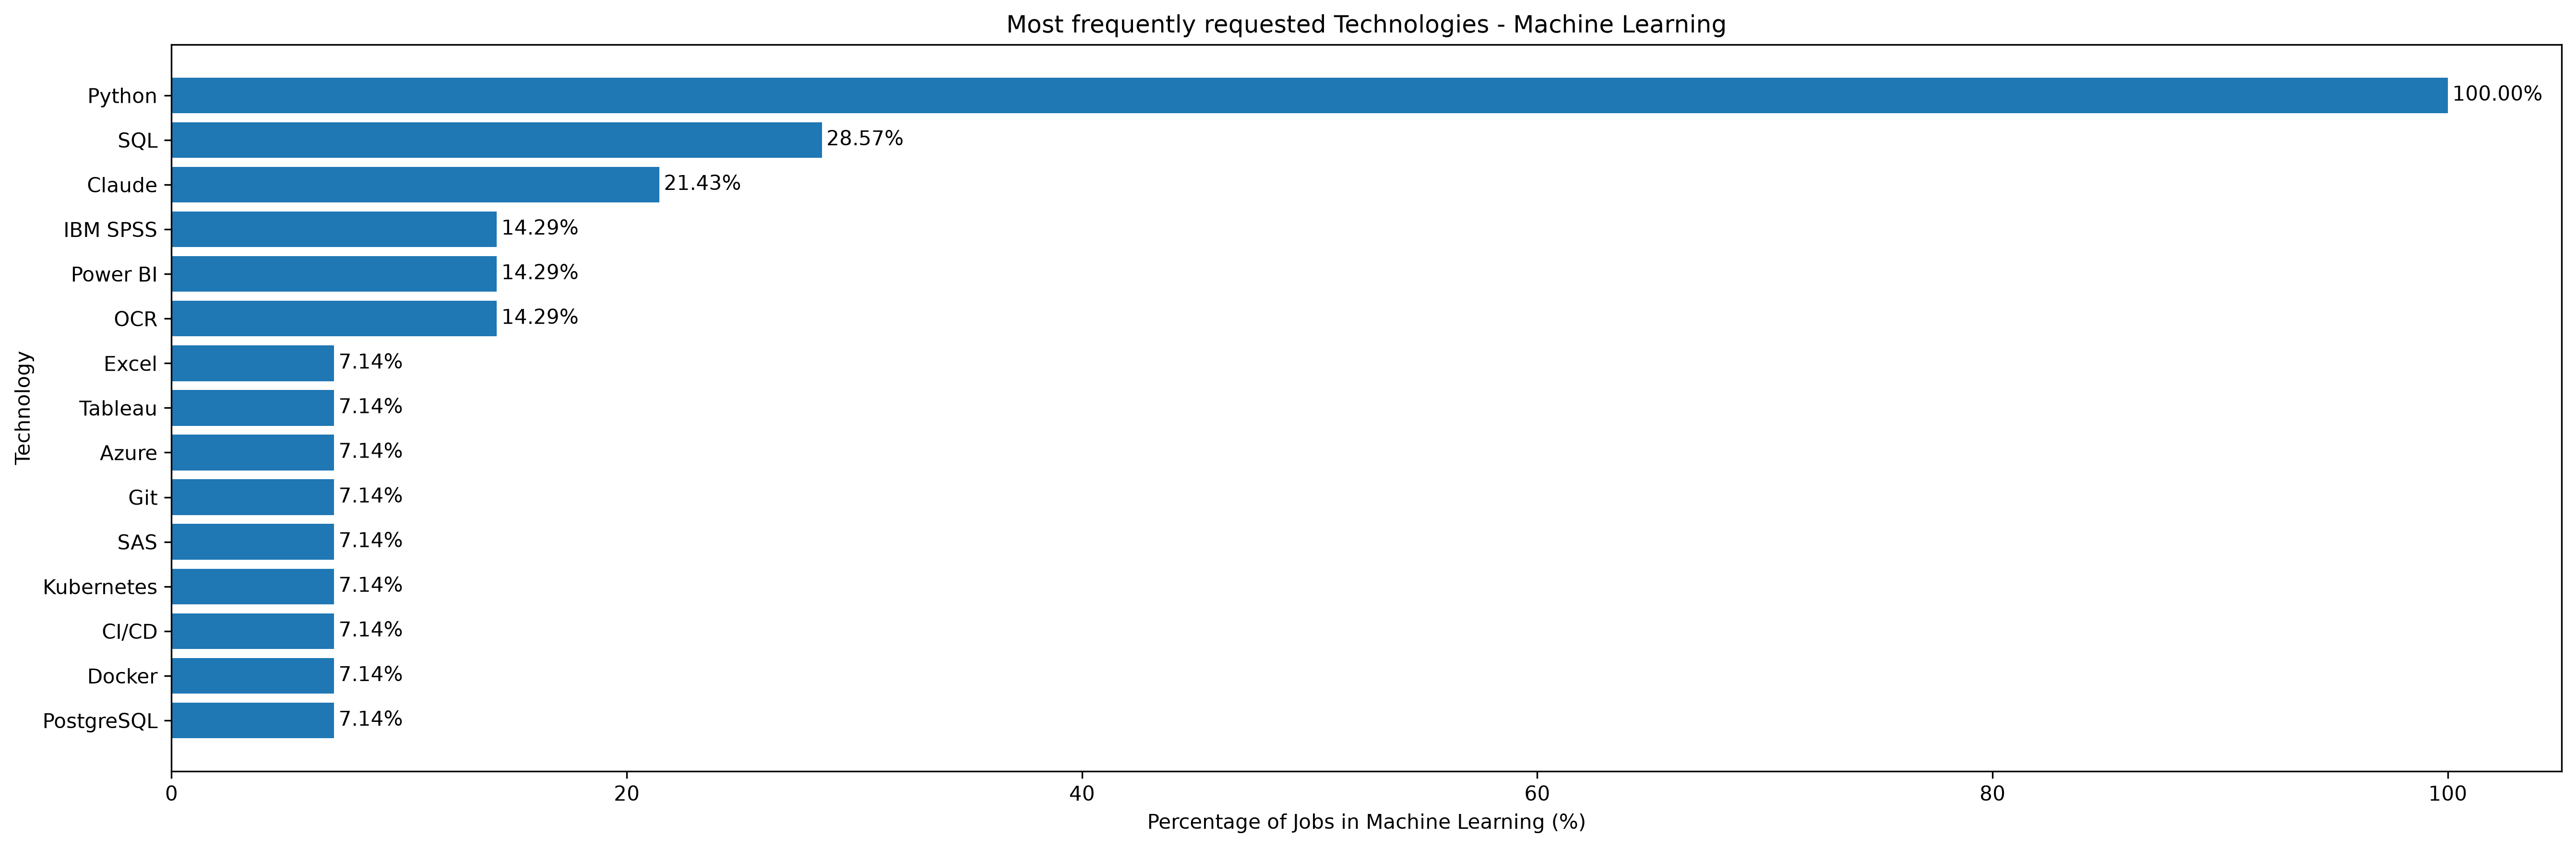
\includegraphics[width=\linewidth]{figures/diagrams/phase2/machine_learning_most_requested_technologies.png}
        \caption{Machine Learning}
        \label{fig:rq3_technologies_machine_learning}
    \end{subfigure}
    \hfill
    \begin{subfigure}{0.48\textwidth}
        \centering
        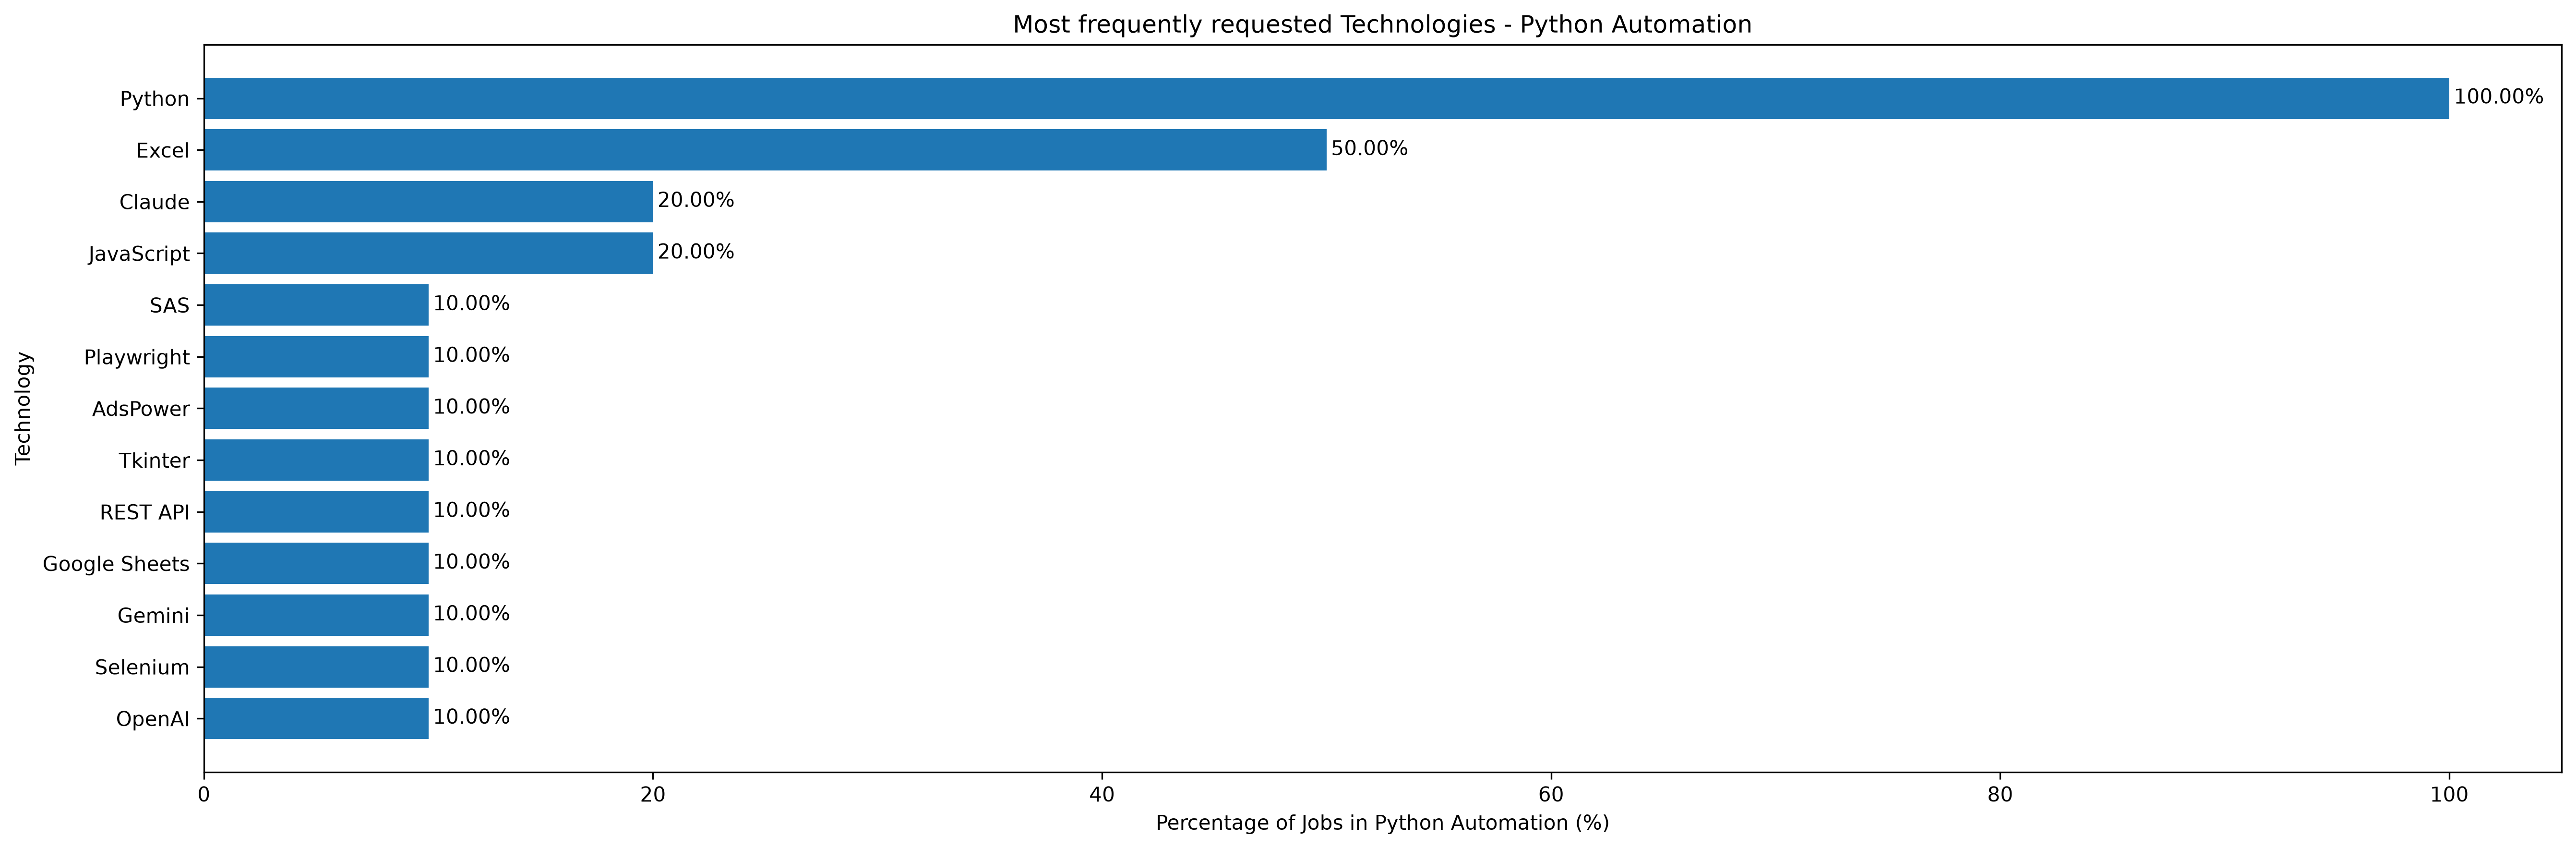
\includegraphics[width=\linewidth]{figures/diagrams/phase2/python_automation_most_requested_technologies.png}
        \caption{Python Automation}
        \label{fig:rq3_technologies_python_automation}
    \end{subfigure}

    \caption{Frequency of technologies and tools within the analysed dataset, overall and by job category. The complete numerical data used to
    generate these figures are available in \texttt{$/data/exports/tables/technologies-summary.csv$}}
    \label{fig:rq3_technologies}
    
\end{figure}

\begin{figure}[H]
    \centering
    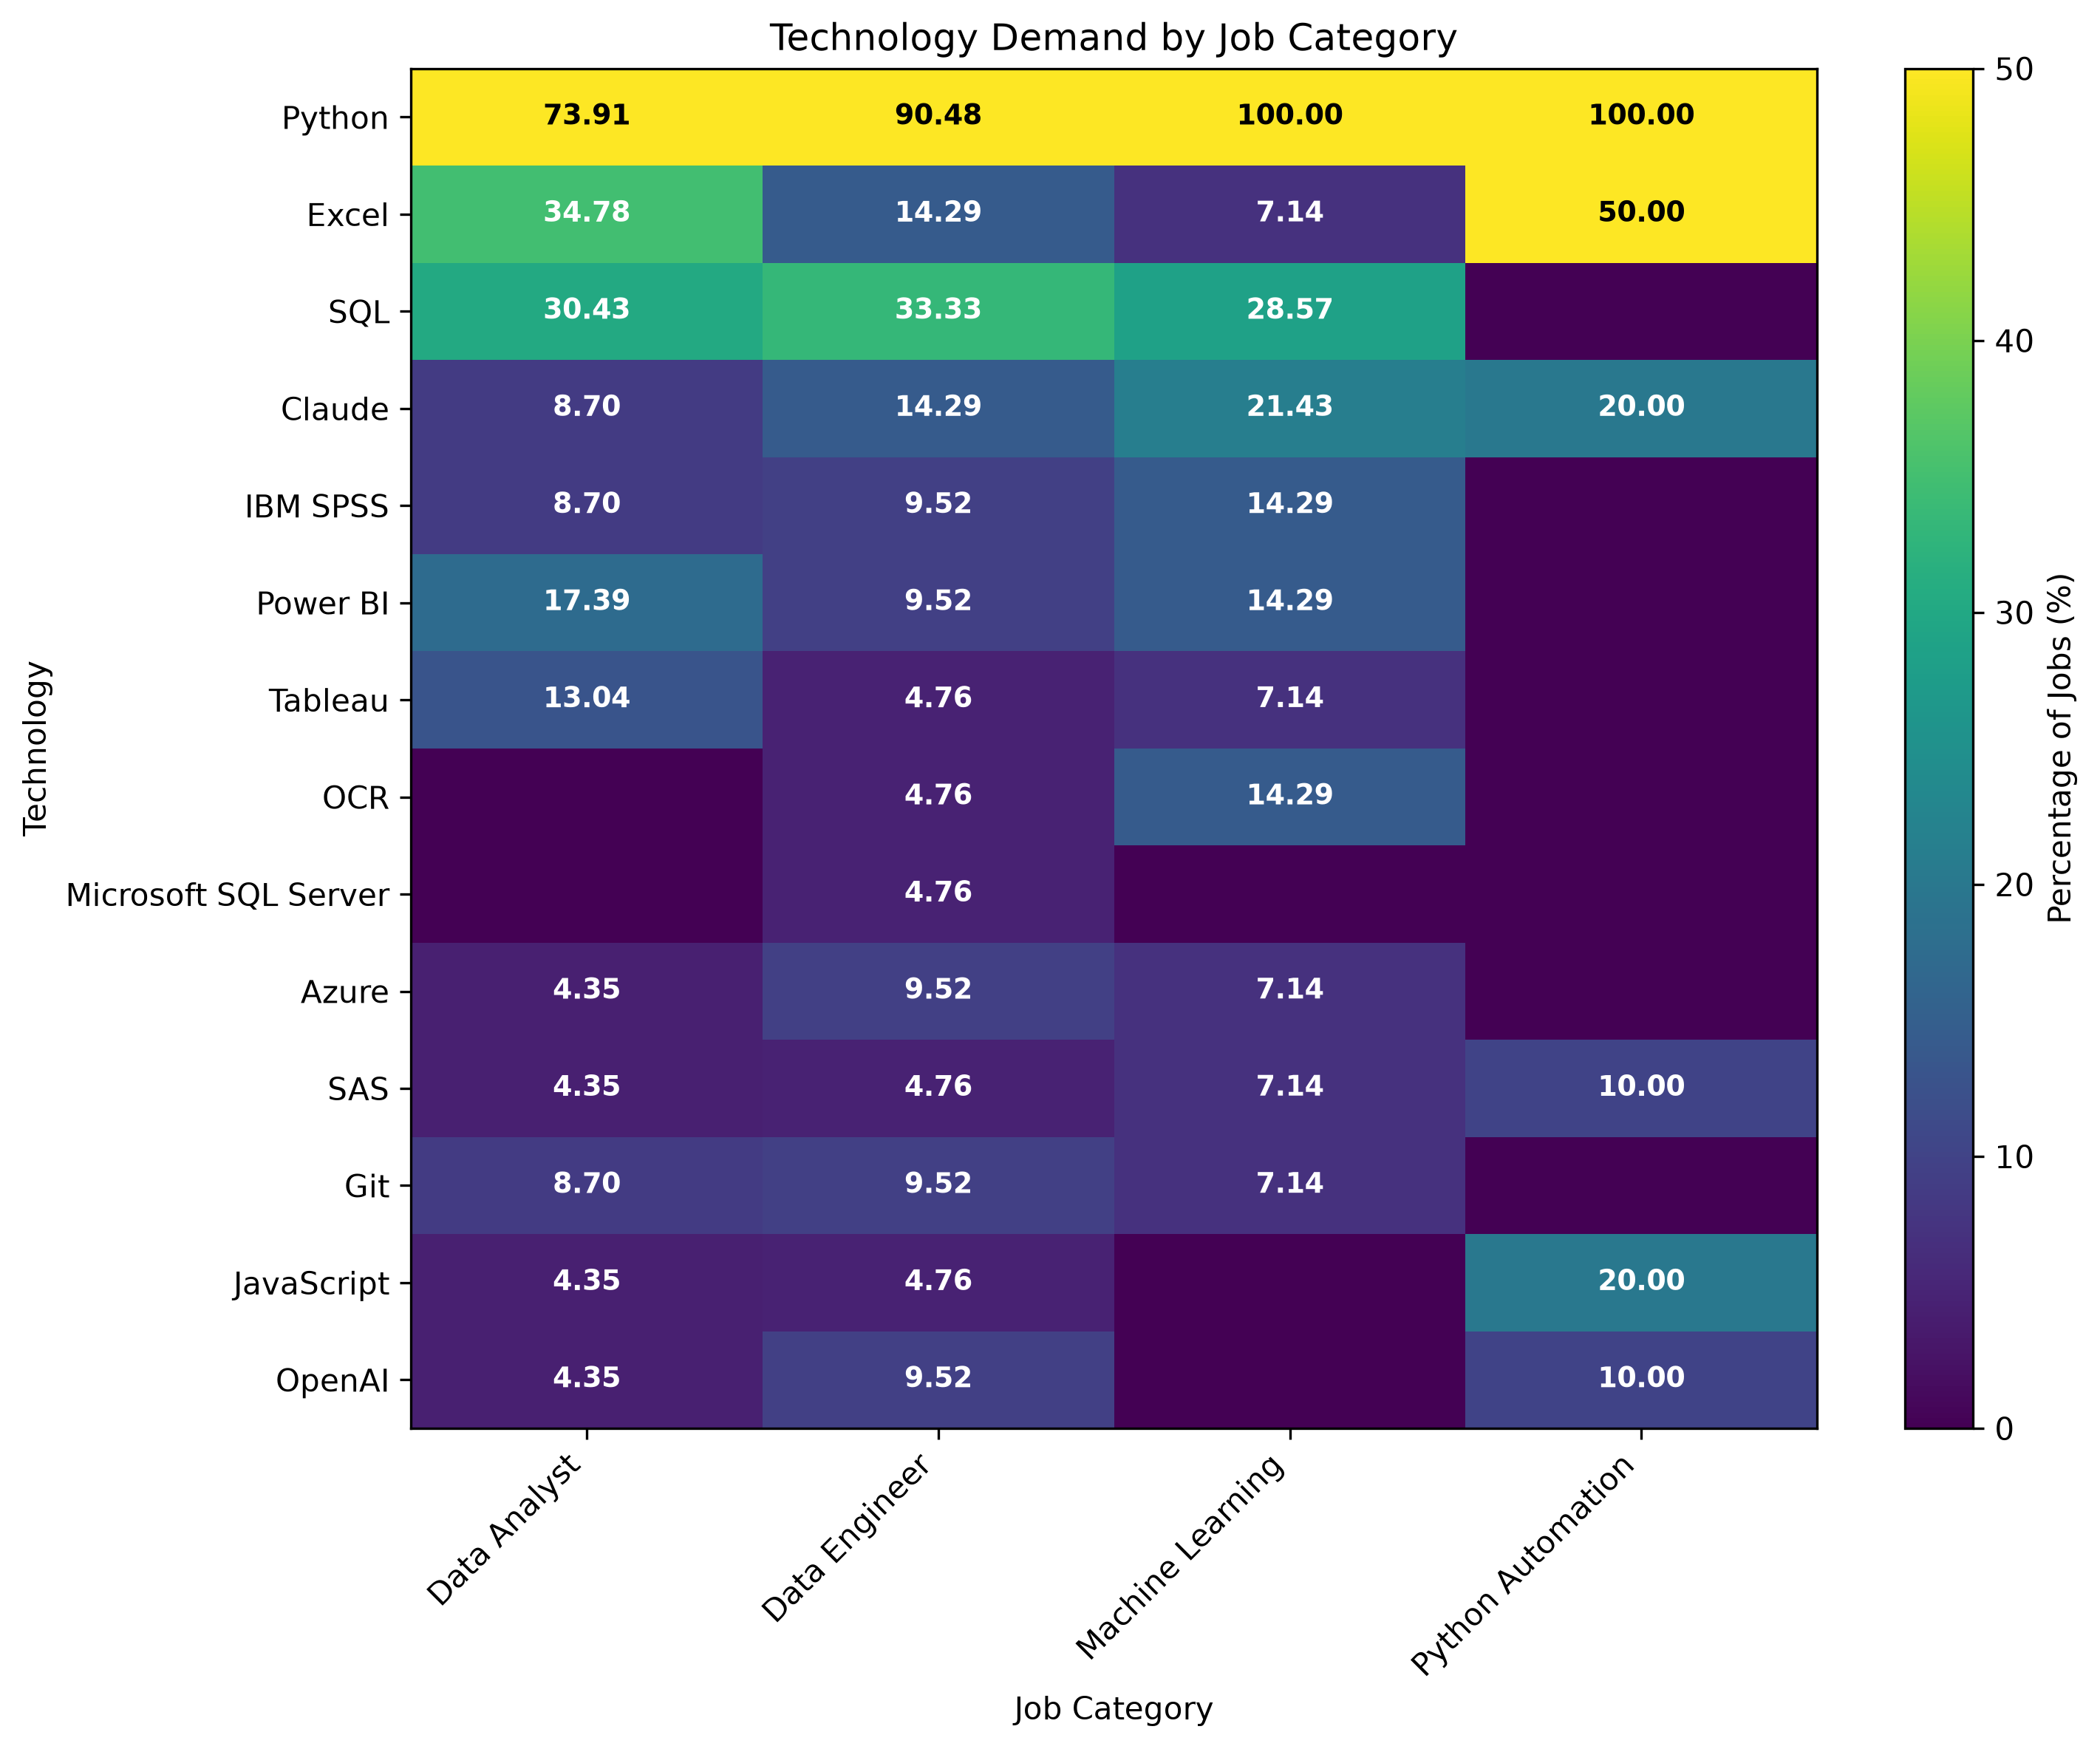
\includegraphics[width=0.75\linewidth]{figures/diagrams/phase2/technology_heatmap_by_category.png}
    \caption{Heatmap of technology and tool usage across different job categories.}
    \label{fig:rq3_technology_heatmap}
\end{figure}

\medskip

\textbf{Results}

The overall distribution of requested technologies is presented in
Figure~\ref{fig:rq3_technologies_overall}. Python was by far the most frequently
requested technology, appearing in more than 84\% of all analysed job
postings. SQL and Microsoft Excel formed the second tier of commonly required
technologies, followed by business intelligence software, AI tools and cloud
services.

Figures~\ref{fig:rq3_technologies_data_analyst}--\ref{fig:rq3_technologies_python_automation} reveal clear differences between
the analysed freelance categories. Data Analyst positions placed strong
emphasis on Python together with Excel, SQL, Power BI and Tableau, reflecting
their focus on data analysis and reporting tasks. Data Engineering jobs
showed the highest demand for SQL and infrastructure-related technologies in
addition to Python, whereas Machine Learning jobs exhibited increased
usage of AI-related tools such as Claude together with OCR software and
statistical packages. Python Automation jobs displayed a different profile,
combining Python with spreadsheet processing, browser automation technologies
and JavaScript.

The heat map shown in Figure~\ref{fig:rq3_technology_heatmap} provides a compact
comparison of these category-specific technology demands. It highlights Python
as the common foundation across all analysed job categories while also
revealing the complementary technologies that distinguish each freelance
specialisation.

\medskip

\textbf{Discussion}

The technology analysis demonstrates that successful freelance Python projects rarely depend on Python alone. Instead, clients typically expect
developers to combine Python programming with additional technologies that are closely related to the application domain.

The observed patterns suggest that Data Analyst roles require strong knowledge of analytical software and reporting tools, Data Engineering
jobs demand database management and data infrastructure skills, while Machine Learning positions increasingly integrate AI platforms and
specialised data processing tools. Python Automation jobs, although smaller in number, frequently combine Python with browser automation
frameworks, APIs and spreadsheet-based workflows.

From the perspective of portfolio development, these findings provide practical guidance for prioritising technical skills. Rather than attempting
to learn a large number of unrelated technologies simultaneously, aspiring freelancers can focus on acquiring the complementary tools that most
frequently accompany Python within their chosen freelance category. Such a targeted learning strategy is likely to increase both portfolio relevance and
competitiveness in the online freelance marketplace.

\section{Research Question 4}

\textbf{Question}

Which combinations of technologies are most frequently requested together?

\medskip

\textbf{Methodology}

To investigate the relationships between requested technologies, every job posting was represented as a set of detected technologies obtained during
the previous analysis. Pairwise co-occurrences were then calculated by counting how frequently two technologies appeared together within the same job
description. The resulting frequencies were normalised by the total number of analysed jobs, and the most frequently occurring technology pairs are
presented in Figure~\ref{fig:technology_pairs}.

\begin{figure}[H]
    \centering
    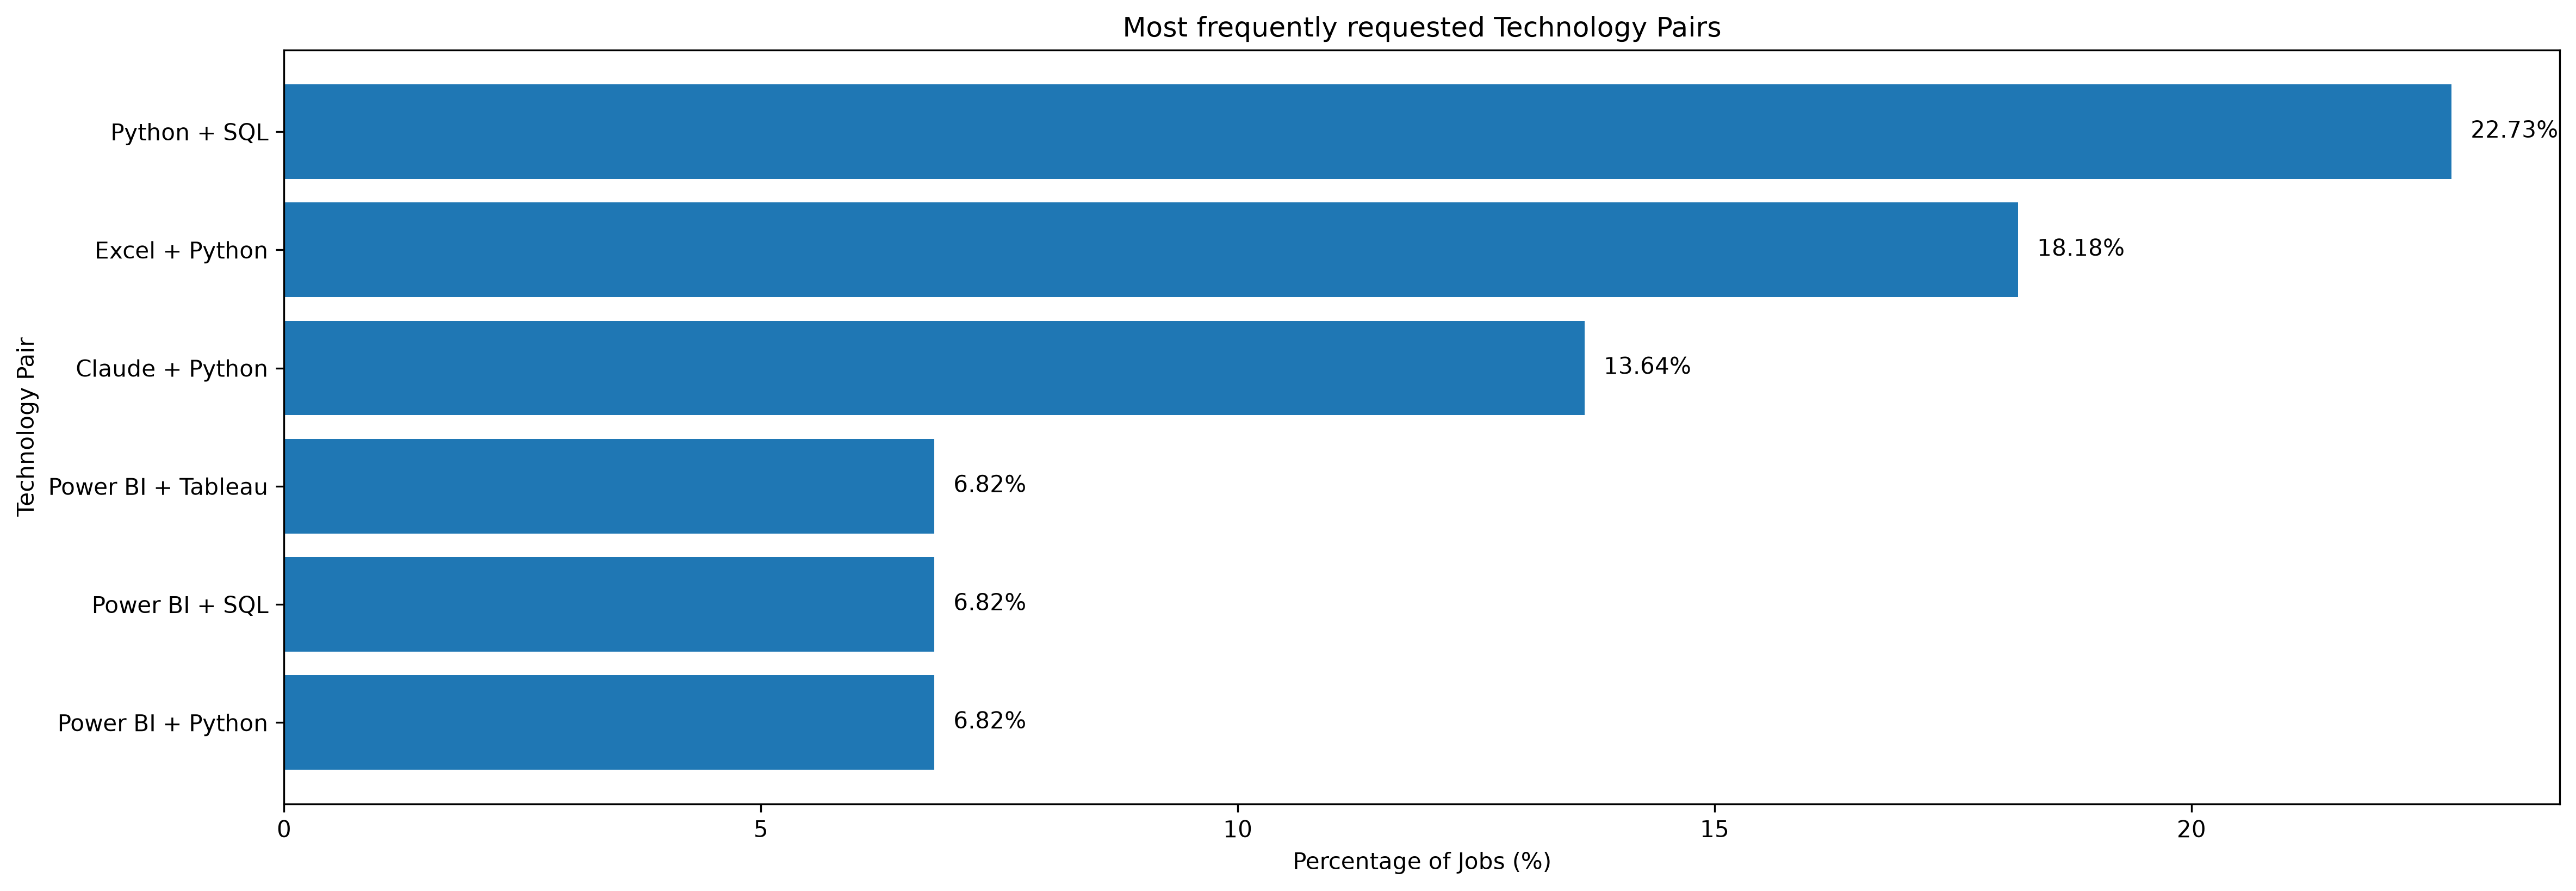
\includegraphics[width=0.75\linewidth]{figures/diagrams/phase2/most_requested_technology_pairs.png}
    \caption{Most frequently requested technology pairs identified in the analysed Upwork job postings. The complete numerical data used to
    generate this figure are available in \texttt{$/data/exports/tables/technology-pairs-summary.csv$}}
    \label{fig:technology_pairs}
\end{figure}

\medskip

\textbf{Results}

The most frequently requested technology combinations are presented in Figure~\ref{fig:technology_pairs}. The pair Python + SQL appeared most often,
being mentioned in almost one quarter of all analysed job postings. The second most common combination was Python + Excel, reflecting the
strong presence of data analysis and reporting tasks within the collected dataset.

Another notable result is the relatively high occurrence of the Python + Claude combination, indicating that AI-assisted workflows have already
become common in Python-related freelance jobs. The remaining technology pairs, including combinations involving Power BI, Tableau and SQL,
occurred considerably less frequently.

\textbf{Discussion}

The co-occurrence analysis demonstrates that employers typically request technology stacks rather than isolated technical skills. Python serves as
the central programming language, but it is most commonly expected together with SQL, spreadsheet software or specialised domain-specific tools.

These findings reinforce the conclusions drawn from the previous research questions. Rather than focusing exclusively on Python itself, aspiring
freelancers should develop complementary technical skills that frequently appear alongside Python in real client jobs. Building a portfolio around
such commonly requested technology combinations is likely to better reflect actual market expectations.

\section{Research Question 5}

\textbf{Question}

What budget ranges and hourly rates are associated with the analysed freelance jobs?

\medskip

\textbf{Methodology}

The pricing information contained in the collected Upwork job postings was analysed separately for fixed-price and hourly projects. For fixed-price
contracts, the reported job budgets were grouped according to the job categories identified in the previous analyses. Likewise, hourly contracts
were grouped according to their advertised hourly rates.

To better understand how compensation changes with required expertise, jobs were additionally grouped by both job category and client-requested
experience level (Entry level, Intermediate and Expert). Boxplots were used to visualise the overall distribution of fixed-price budgets and
hourly rates, while heatmaps summarise the median compensation for each job category and experience level. Median values were preferred over
arithmetic means because they are less sensitive to extreme outliers, which are common in freelance marketplace data.

The distributions of fixed-price budgets are presented in Figures~\ref{fig:fixed_budget_distribution} and \ref{fig:fixed_budget_heatmap},
while hourly-rate statistics are shown in Figures~\ref{fig:hourly_distribution} and \ref{fig:hourly_heatmap}.

\begin{figure}[H]
    \centering

    % első ábra
    \begin{subfigure}{0.75\textwidth}
        \centering
        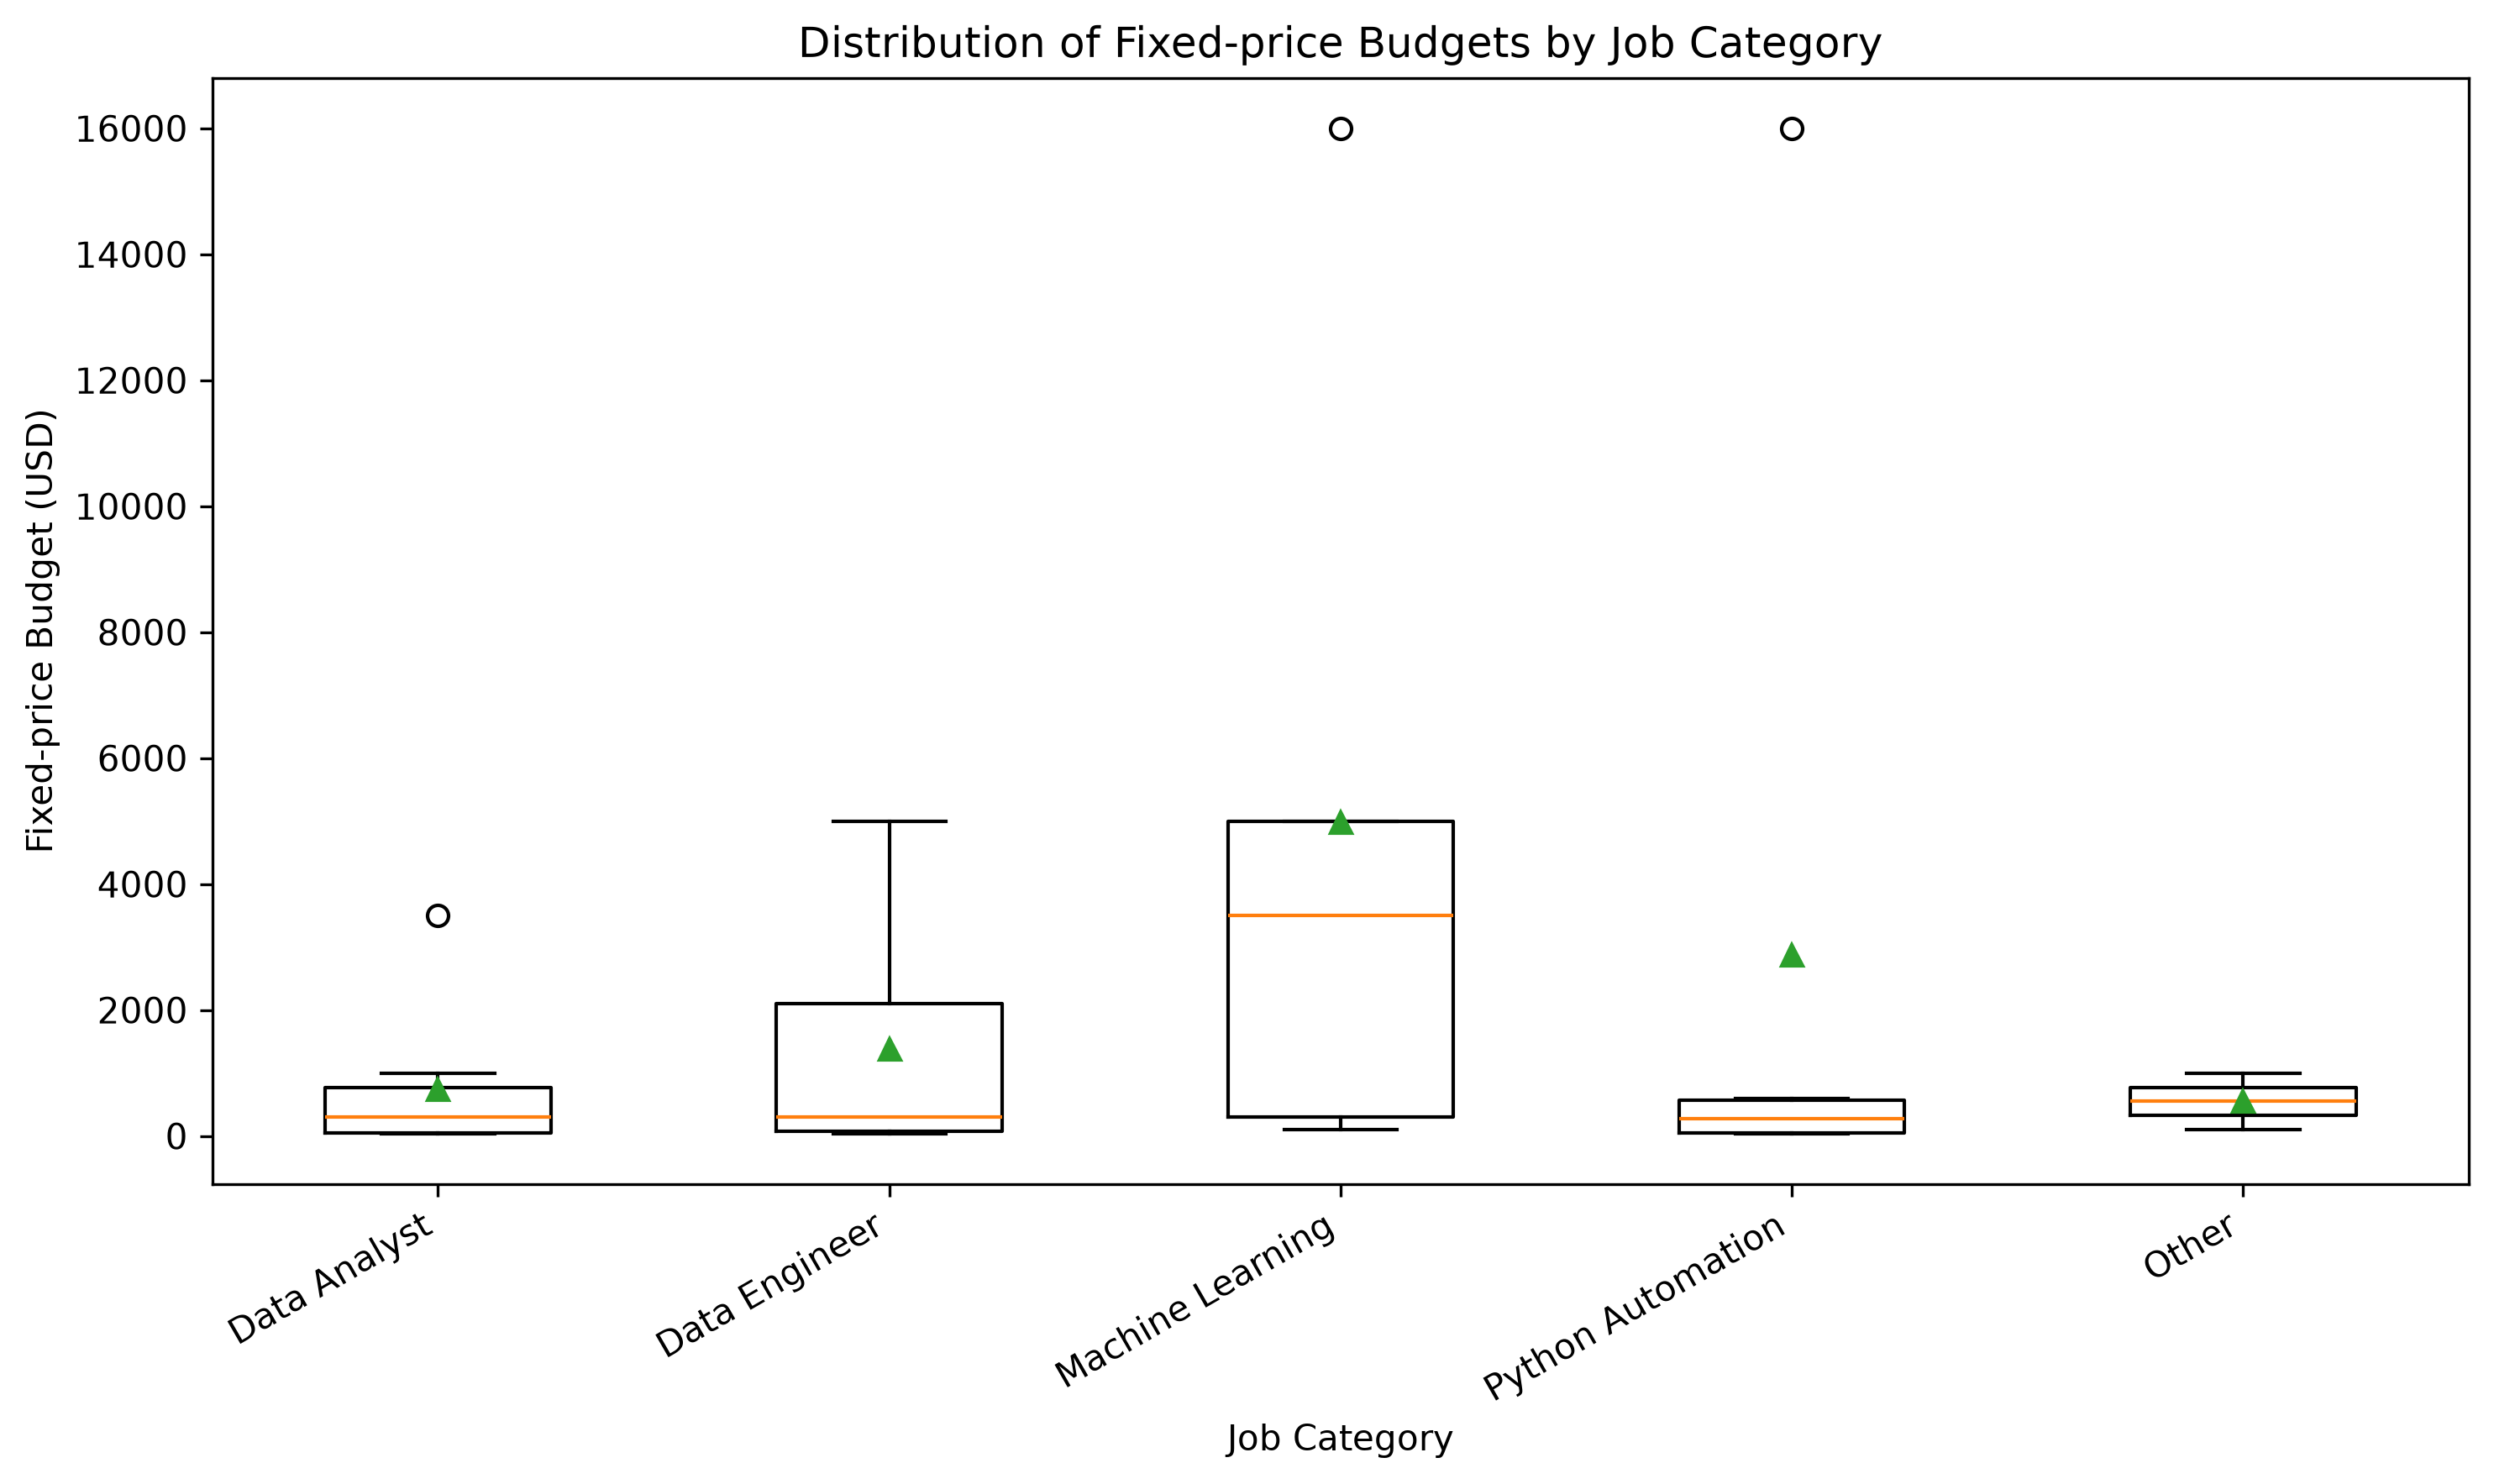
\includegraphics[width=\linewidth]{figures/diagrams/phase2/fixed_price_budget_distribution.png}
        \caption{Distribution of fixed-price budgets by job category.}
        \label{fig:fixed_budget_distribution}
    \end{subfigure}

    \vspace{0.5cm}

    % második sor
    \begin{subfigure}{0.75\textwidth}
        \centering
        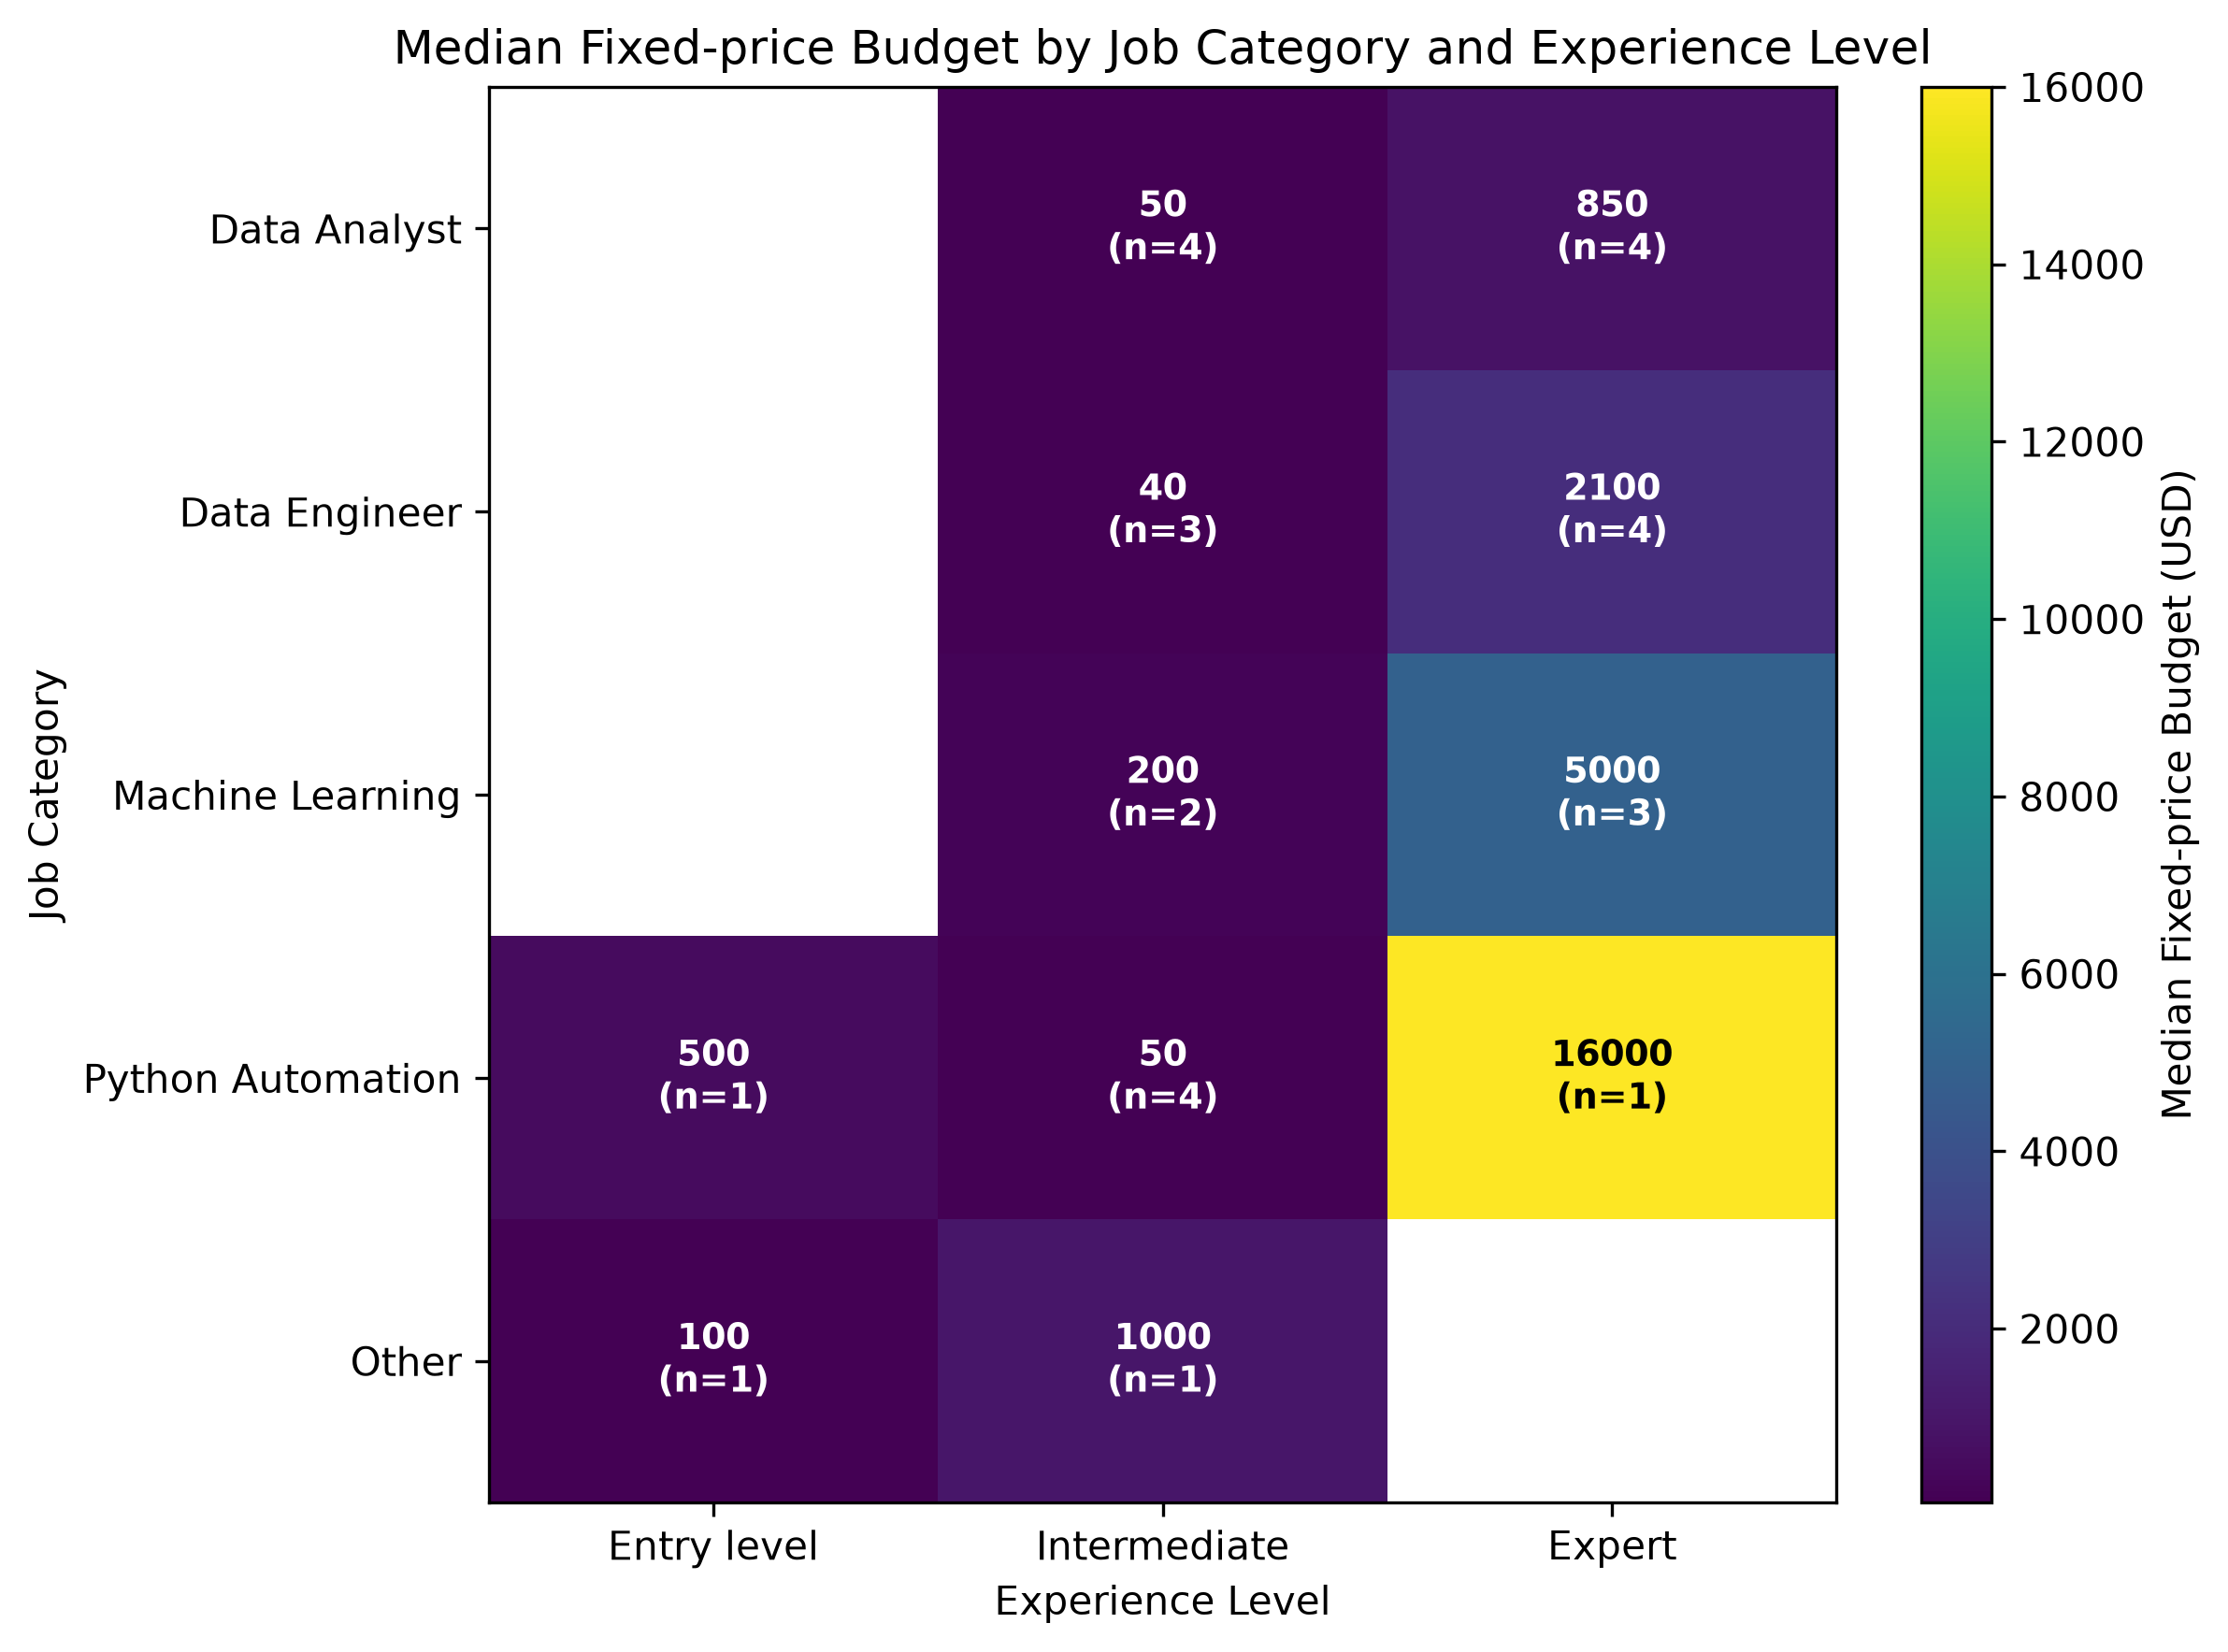
\includegraphics[width=\linewidth]{figures/diagrams/phase2/fixed-price_budget_heatmap.png}
        \caption{Median fixed-price budgets by job category and experience level.}
        \label{fig:fixed_budget_heatmap}
    \end{subfigure}

    \vspace{0.5cm}

    \caption{Budget and hourly rate distributions within the analysed dataset, overall and by job category and experience level.
    The complete numerical data used to generate these figures are available in \texttt{$/data/exports/tables/fixed-budget-summary.csv$}}
    \label{fig:fixed_budget_figures}
\end{figure}

\begin{figure}
    \centering
    % első ábra
    \begin{subfigure}{0.75\textwidth}
        \centering
        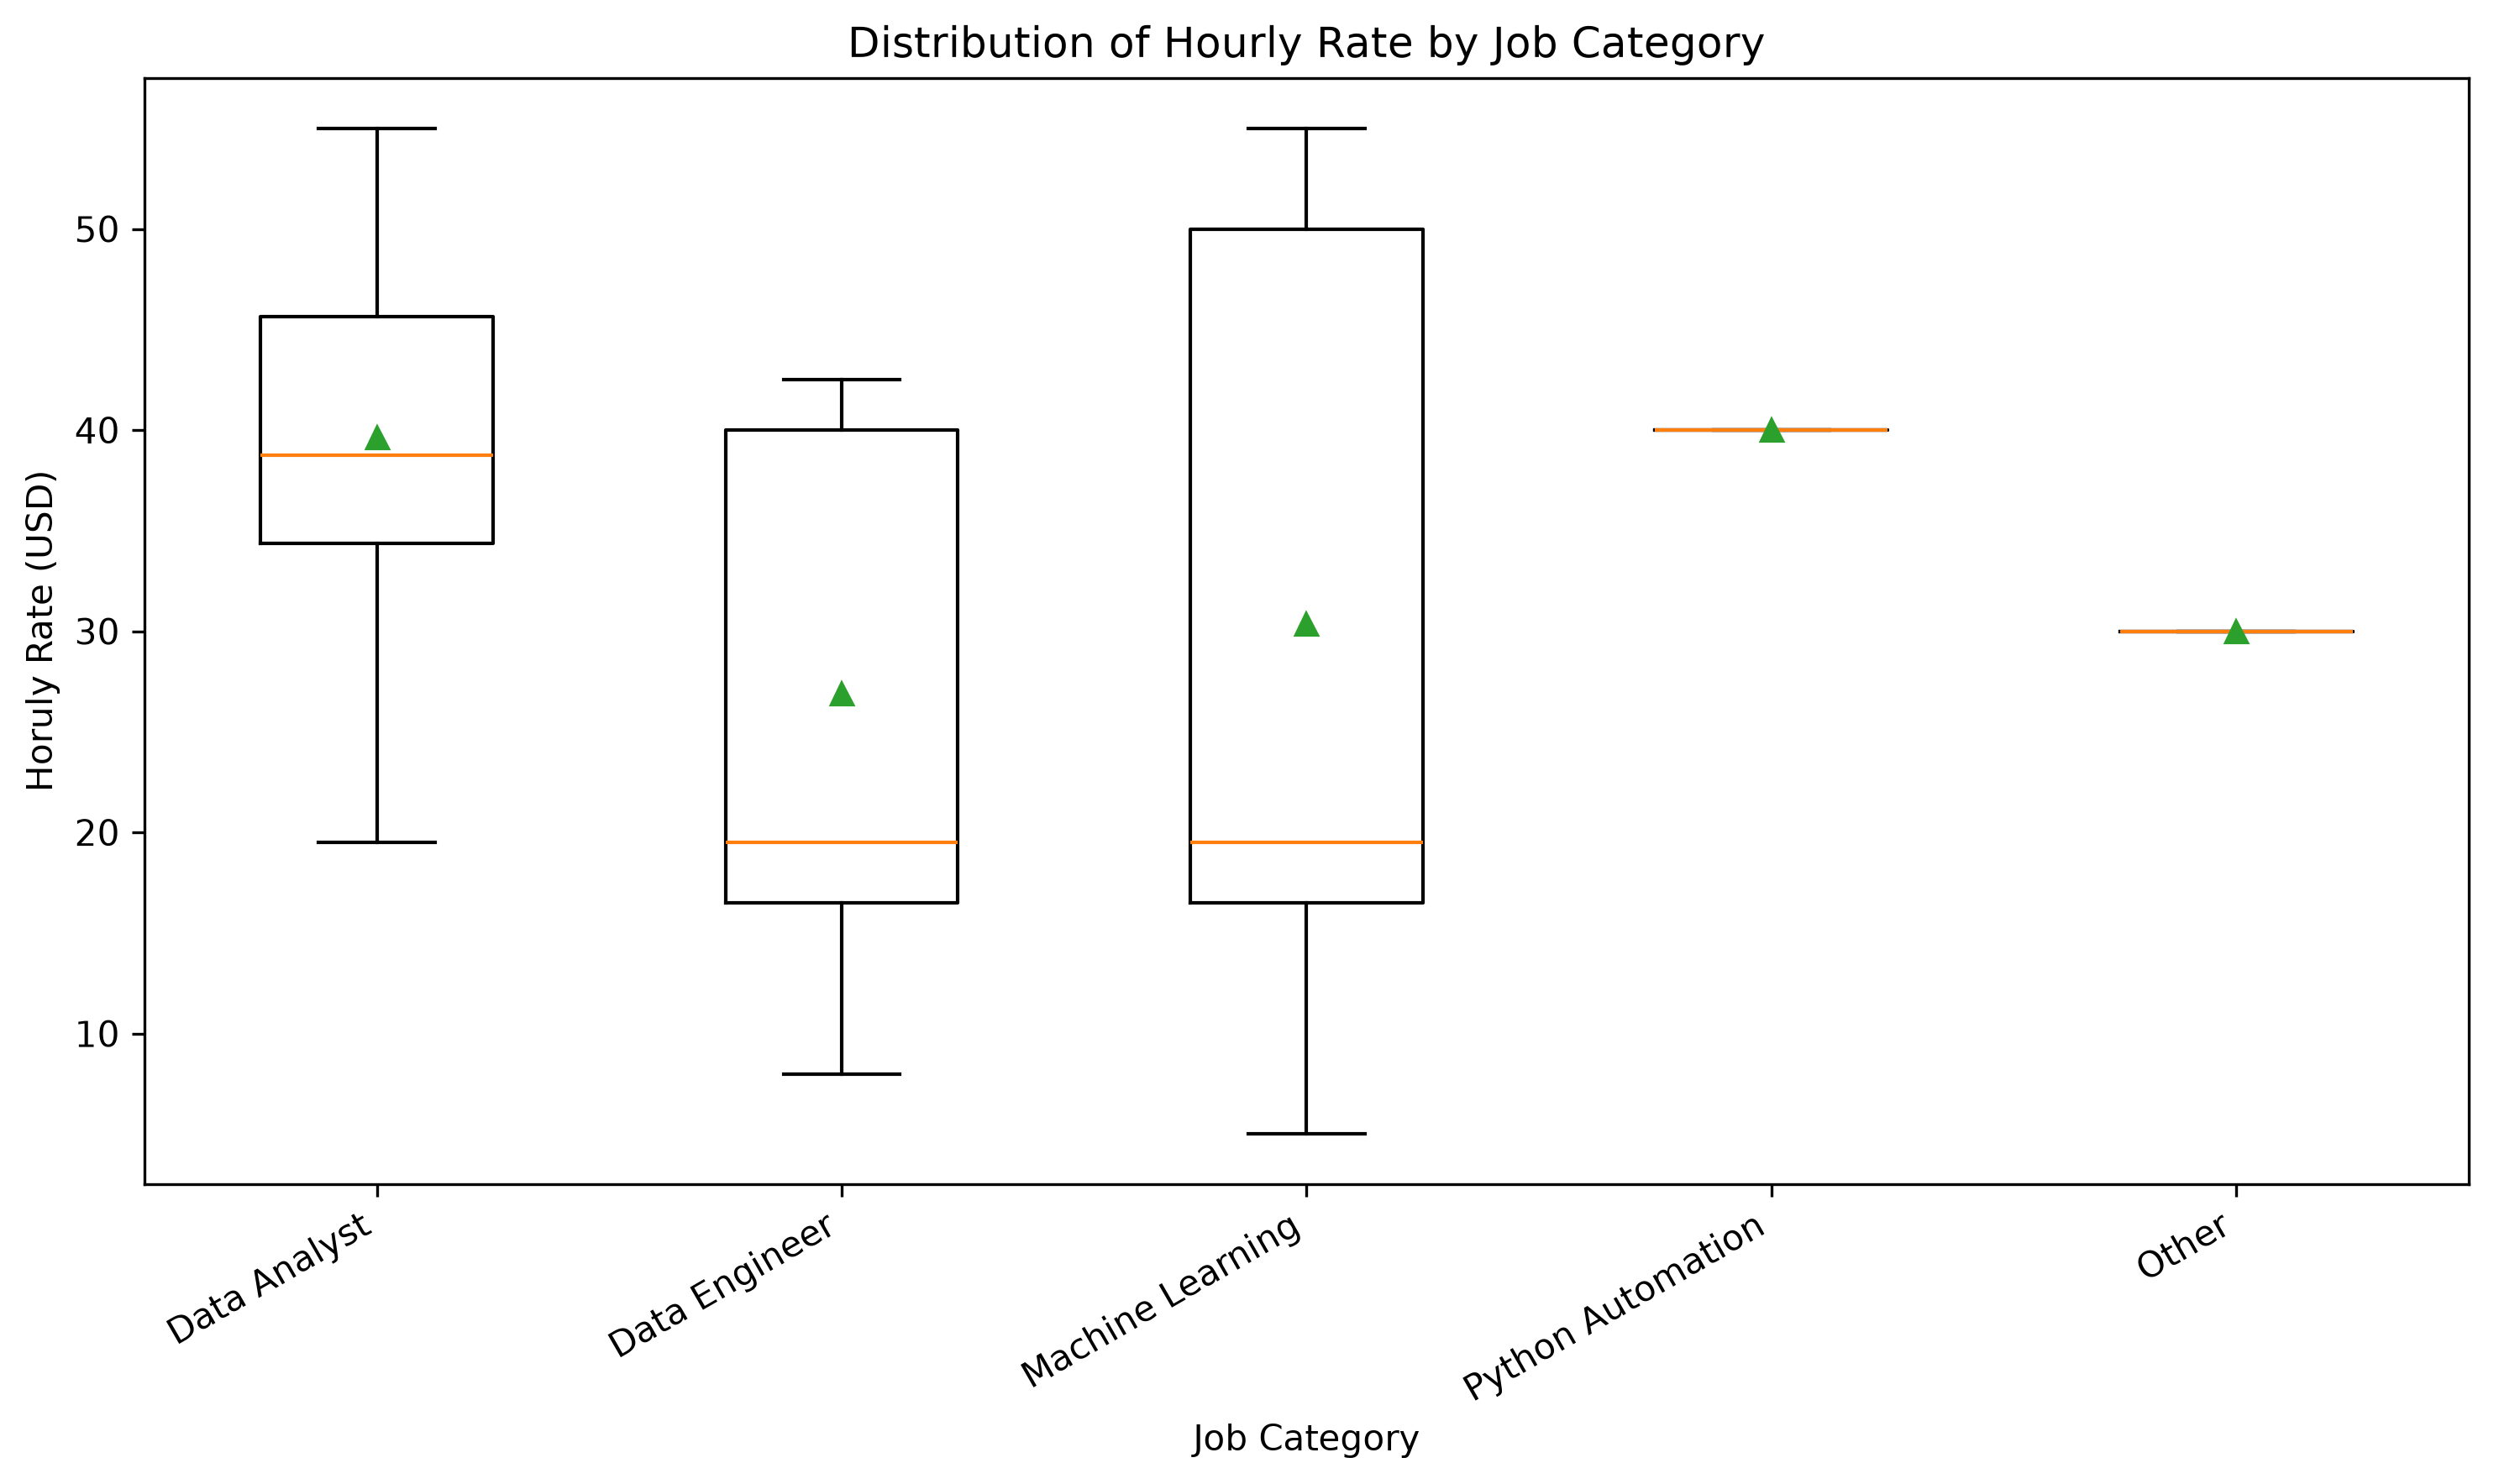
\includegraphics[width=\linewidth]{figures/diagrams/phase2/hourly_budget_distribution.png}
        \caption{Distribution of hourly rates by job category.}
        \label{fig:hourly_distribution}
    \end{subfigure} 

    \vspace{0.5cm}

    % második sor
    \begin{subfigure}{0.75\textwidth}
        \centering
        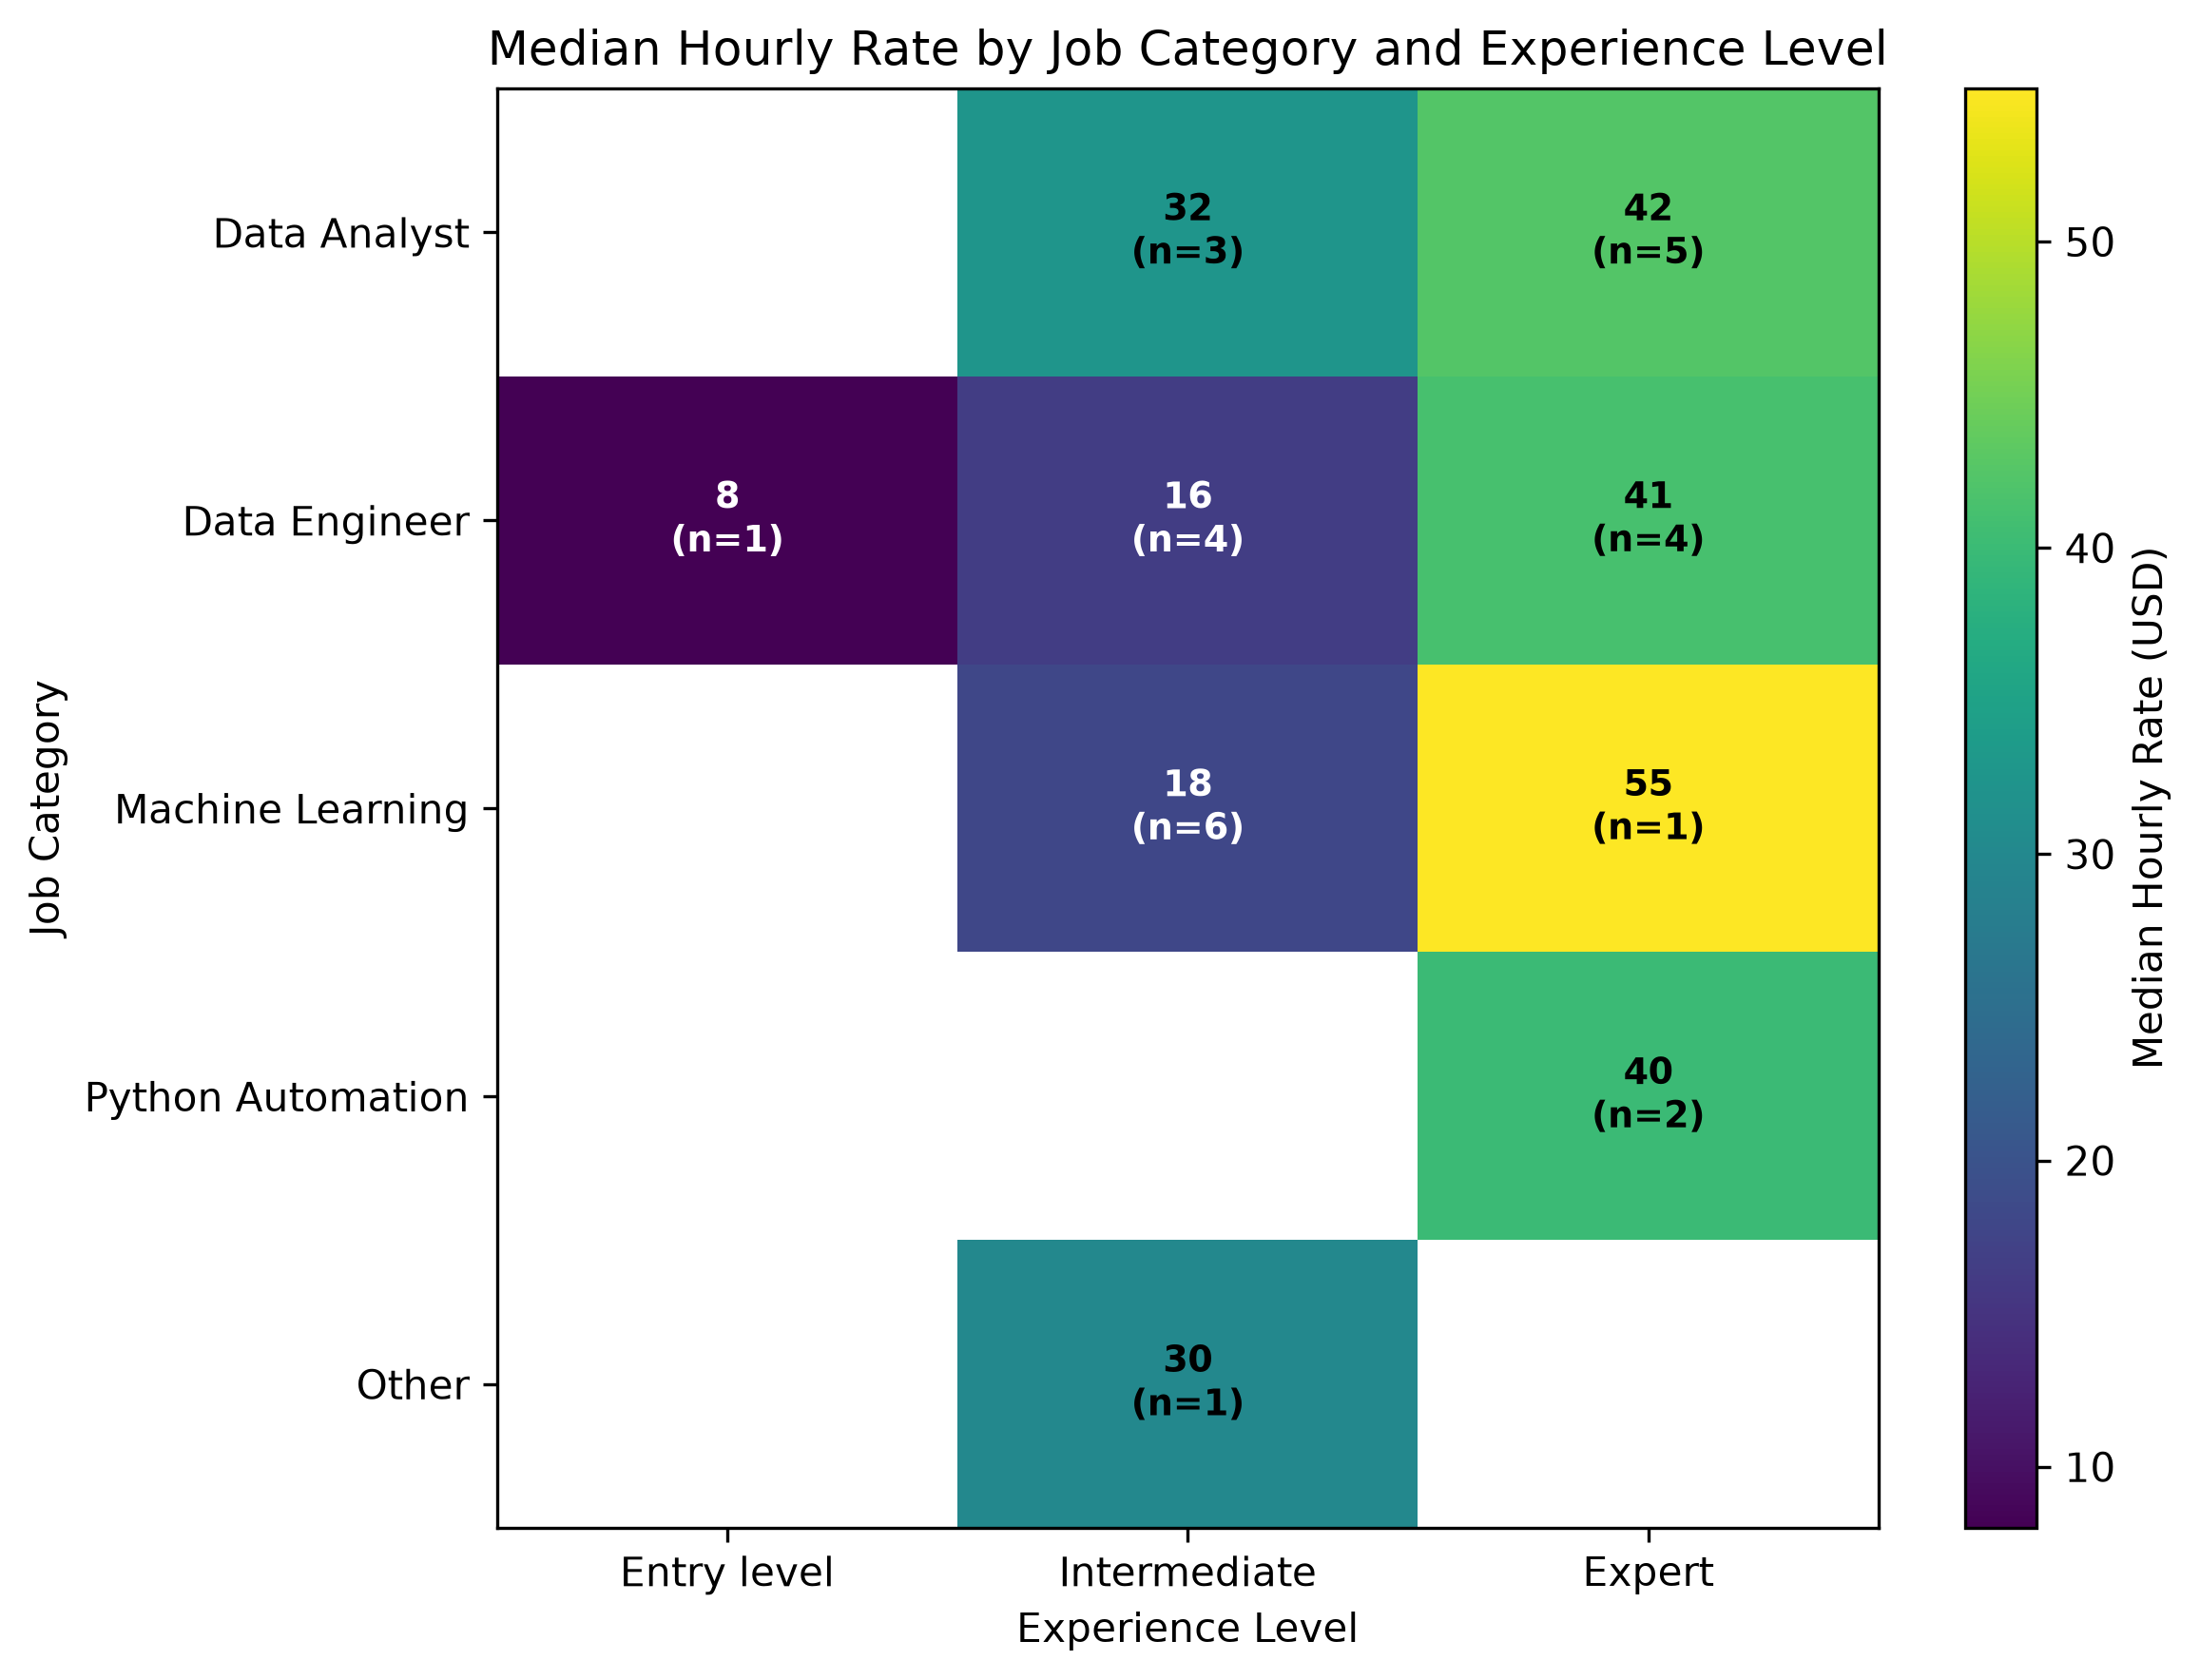
\includegraphics[width=\linewidth]{figures/diagrams/phase2/hourly_budget_heatmap.png}
        \caption{Median hourly rates by job category and experience level.}
        \label{fig:hourly_heatmap}
    \end{subfigure}
    
    \caption{Budget and hourly rate distributions within the analysed dataset, overall and by job category and experience level.
    The complete numerical data used to generate these figures are available in \texttt{$/data/exports/tables/hourly-budget-summary.csv$}}
    \label{fig:hourly_figures}
\end{figure}

\medskip

\textbf{Results}

\subsubsection*{Results}

The fixed-price budget distributions shown in Figures~\ref{fig:fixed_budget_distribution} and \ref{fig:fixed_budget_heatmap} reveal substantial
differences between job categories. Machine Learning jobs generally command the highest budgets, with expert-level jobs having a median fixed price of
\$5000. Data Engineer jobs also exhibit relatively high budgets, reaching a median of \$2100 for expert-level work, whereas expert-level Data Analyst
jobs have a considerably lower median budget of \$850.

The hourly-rate analysis presented in Figures~\ref{fig:hourly_distribution} and \ref{fig:hourly_heatmap} shows a similar trend. Expert-level
jobs are consistently associated with higher hourly rates than intermediate or entry-level work. The highest observed median hourly rate is \$55 for
expert Machine Learning jobs, followed by approximately \$42 for expert Data Analyst jobs and \$41 for expert Data Engineer jobs. Python
Automation jobs advertise hourly rates around \$40 for expert-level work.

Across both pricing models, increasing experience requirements are associated with substantially higher client budgets, although several categories
contain only a limited number of observations and should therefore be interpreted with appropriate caution.

\medskip

\textbf{Discussion}

The pricing analysis indicates that both job complexity and required expertise strongly influence freelance compensation. Machine Learning jobs
offer the highest potential earnings, particularly for experienced freelancers, while Data Engineering jobs also command relatively high
budgets. Data Analysis jobs appear more numerous but generally offer lower fixed-price compensation.

The results further demonstrate that experience level has a considerable effect on pricing regardless of job category. Expert-level jobs
consistently receive substantially larger budgets and higher hourly rates than intermediate or entry-level work.

However, the pricing heatmaps should be interpreted with caution. The analysis is based on a dataset containing only 44 job postings, and
after splitting the data simultaneously by job category and experience level, several cells contain only one or two observations. 
Consequently, individual median values may be strongly influenced by a single job and should therefore not be interpreted as
representative market prices.

Nevertheless, despite the limited sample size, the overall trends remain consistent across both the fixed-price and hourly-rate analyses. The results
suggest that jobs requiring higher levels of expertise generally command substantially higher compensation, while Machine Learning and
Data Engineering appear to represent the highest-value specialisations within the analysed dataset.

\section[Phase 2 Summary]{Phase Summary}

The analyses performed in this phase provide a comprehensive description of the analysed Python freelance market. Together, the five
research questions examined market demand from complementary perspectives, including job category distribution, required Python packages,
broader technology stacks, commonly requested technology combinations, and project pricing. Rather than drawing practical recommendations,
the objective of this phase was to establish a reliable empirical foundation based on real Upwork job postings. These findings form the basis for
the next phase, where the collected evidence will be synthesised into actionable market insights.